\chapter{矢量分析}
\markboth{矢量分析}{矢量分析}

\begin{remark}[本章定位与阅读约定]\label{rem:vector_analysis_chapter_positioning}
矢量分析研究标量场与矢量场的微分与积分运算。本章严格建立梯度、散度、旋度三个算子的理论体系，证明乘积法则、基本恒等式与积分定理，并讨论向量场的分类、势函数存在性与正交曲线坐标系中的算子表达式。

\textbf{阅读约定。}本章默认空间与时间连续，离散格点模型在「周期流形」章讨论。凡陈述涉及定义域时，一律显式给出该定义域的正则性条件（开集、单连通、正则边界或正则有界区域之一），凡涉及可微性时，一律显式给出所要求的连续可微阶数。凡结论依赖附加假设者，该假设在陈述中逐条列出；凡目前只有启发性论证而无可陈述之定理者，一律标注为「研究纲领」或「待研究问题」，不作为已证结论使用。
\end{remark}

\begin{figure}[htbp]
\centering
\begin{tikzpicture}[
  font=\small,
  box/.style={draw, rounded corners, fill=blue!8, minimum width=2.6cm, minimum height=0.8cm, align=center},
  sub/.style={draw, rounded corners, fill=green!10, minimum width=2.4cm, minimum height=0.7cm, align=center, font=\footnotesize},
  arr/.style={->, thick, >=stealth}
]
  \node[box] (field) {标量场与矢量场\\定义域与正则性};
  \node[box, right=1.0cm of field] (ops) {三个微分算子\\梯度/散度/旋度};
  \node[box, right=1.0cm of ops] (rules) {乘积法则\\基本恒等式};
  \node[box, right=1.0cm of rules] (integral) {积分定理\\格林/斯托克斯/高斯};
  \node[sub, below=1.0cm of field] (class) {向量场分类\\无旋/无散/调和};
  \node[sub, below=1.0cm of ops] (potential) {势函数\\标量势/矢量势};
  \node[sub, below=1.0cm of rules] (helmholtz) {亥姆霍兹分解\\无旋+无散};
  \node[sub, below=1.0cm of integral] (curvilinear) {正交曲线坐标\\算子表达式};
  \node[box, fill=orange!12, below=1.0cm of $(class)!0.5!(curvilinear)$] (unify) {向量场结构统一：分类、分解、坐标表达};
  \draw[arr] (field) -- (ops);
  \draw[arr] (ops) -- (rules);
  \draw[arr] (rules) -- (integral);
  \draw[arr] (field) -- (class);
  \draw[arr] (ops) -- (potential);
  \draw[arr] (rules) -- (helmholtz);
  \draw[arr] (integral) -- (curvilinear);
  \draw[arr] (class) -- (unify);
  \draw[arr] (potential) -- (unify);
  \draw[arr] (helmholtz) -- (unify);
  \draw[arr] (curvilinear) -- (unify);
\end{tikzpicture}
\caption{本章结构总览：从标量场与矢量场出发，经三个微分算子、乘积法则与基本恒等式，到积分定理、向量场分类、势函数、亥姆霍兹分解与正交曲线坐标系，最终统一于向量场结构。}
\label{fig:vector_analysis_overview}
\end{figure}

\section{标量场与矢量场}

本节固定全部后续讨论的对象与定义域。这里给出的正则性条件并非技术性的装饰：本章若干结论（如散度定理、势函数存在性）在定义域不满足相应条件时确实失效，\cref{ex:slit_domain_counterexample} 与 \cref{ex:needle_domain} 给出两个反例。

\begin{definition}[标量场]\label{def:scalar_field}
设 $\mathcal{M} \subseteq \mathbb{R}^n$ 为非空开集，$n \in \{1,2,3\}$（本章主要讨论 $n=3$；二维情形 $n=2$ 可由同一套算子理论逐点退化得到）。一个\textbf{标量场}是一个函数
\[
f: \mathcal{M} \to \mathbb{R}, \qquad \mathbf{x} = (x_1, \dots, x_n) \mapsto f(\mathbf{x}).
\]
若 $f$ 在 $\mathcal{M}$ 上具有直到 $k$ 阶的连续偏导数，则记 $f \in C^k(\mathcal{M})$；特别地 $C^0(\mathcal{M})$ 表示 $\mathcal{M}$ 上的连续函数全体。

\textbf{前提与约定}：当 $k \ge 1$ 时，$f \in C^k(\mathcal{M})$ 蕴含 $f$ 在 $\mathcal{M}$ 上处处可微（连续偏导数存在即蕴含可微），故下文所有对 $f$ 使用链式法则、方向导数公式与泰勒展开之处，$k \ge 1$ 的假设均足以支持。若 $f$ 只在 $\mathcal{M}$ 的某个子集上定义，则该子集必须显式给出。
\end{definition}

\begin{definition}[矢量场]\label{def:vector_field}
设 $\mathcal{M} \subseteq \mathbb{R}^3$ 为非空开集。一个\textbf{矢量场}是一个向量值函数
\[
\mathbf{F}: \mathcal{M} \to \mathbb{R}^3, \qquad
\mathbf{F}(\mathbf{x}) = \bigl(F_1(\mathbf{x}),\, F_2(\mathbf{x}),\, F_3(\mathbf{x})\bigr),
\]
其中 $F_i: \mathcal{M} \to \mathbb{R}$（$i=1,2,3$）称为 $\mathbf{F}$ 的\textbf{分量函数}。若所有 $F_i \in C^k(\mathcal{M})$，则记 $\mathbf{F} \in C^k(\mathcal{M}, \mathbb{R}^3)$。

\textbf{约定}：$\mathbf{F} \in C^k(\mathcal{M},\mathbb R^3)$ 按定义等价于三个分量函数都属于 $C^k(\mathcal{M})$；本章所有对矢量场的可微性要求均逐分量施加，不再重复说明。
\end{definition}

\begin{definition}[闭包、边界、正则区域]\label{def:field_domain}
设 $\mathcal{M} \subseteq \mathbb{R}^3$ 为非空开集。其\textbf{闭包}记为 $\overline{\mathcal{M}}$，\textbf{边界}记为 $\partial \mathcal{M} = \overline{\mathcal{M}} \setminus \mathcal{M}$。若 $\partial \mathcal{M}$ 是分片光滑曲面，则称 $\mathcal{M}$ 具有\textbf{正则边界}。特别地，若 $\mathcal{M}$ 有界、$\overline{\mathcal M}$ 是紧集，且 $\partial \mathcal{M}$ 是有限个不相交的光滑闭曲面的并，则称 $\mathcal{M}$ 为\textbf{正则区域}（等价地：$\mathcal{M}$ 有界连通、边界分片光滑且不含尖点与自交）。

\textbf{三项用途}：正则区域是散度定理（\cref{thm:divergence}）成立的自然定义域；分片光滑有向曲面及其分段光滑边界是旋度定理（\cref{thm:stokes}）成立的自然定义域；单连通性是势函数存在性（\cref{thm:irrotational_potential}）成立的必要附加条件。
\end{definition}

\begin{example}[两个基本标量场与矢量场]
温度分布 $T(x,y,z)$ 是标量场：在空间旋转下，某点的温度数值不变。风速场 $\mathbf{v}(x,y,z)$ 是矢量场：在空间旋转下，其分量按旋转矩阵变换。二者的本质区别不在于「是否带方向」，而在于\textbf{在坐标变换下的变换律}——这一点在 \cref{sec:trans_scale_rotate} 中会被精确化。
\end{example}

\begin{figure}[htbp]
\centering
\begin{tikzpicture}[scale=0.9,>=stealth]
  % 标量场
  \begin{scope}[shift={(0,0)}]
    \foreach \r in {0.4,0.8,1.2,1.6,2.0}{
      \draw[gray!50] (0,0) circle (\r);
    }
    \node[font=\footnotesize] at (0,-2.4) {(a) 标量场 $f$：等值线};
    \filldraw[blue] (0.8,0.6) circle (2pt);
    \draw[->,thick,blue] (0.8,0.6) -- (1.3,1.0) node[right,font=\footnotesize]{$\nabla f$};
  \end{scope}
  % 矢量场
  \begin{scope}[shift={(5,0)}]
    \foreach \x in {-1.5,-0.75,0,0.75,1.5}{
      \foreach \y in {-1.5,-0.75,0,0.75,1.5}{
        \pgfmathsetmacro{\vx}{-\y}
        \pgfmathsetmacro{\vy}{\x}
        \draw[->,thick,red,>=stealth] (\x,\y) -- ({\x+0.3*\vx},{\y+0.3*\vy});
      }
    }
    \node[font=\footnotesize] at (0,-2.4) {(b) 矢量场 $\mathbf F$：箭头表示方向与大小};
  \end{scope}
\end{tikzpicture}
\caption{标量场与矢量场的直观对比：标量场用等值线表示，矢量场用箭头表示。}
\label{fig:scalar_vector_field}
\end{figure}

\begin{example}[定义域假设不可省：带缝平面的反例]\label{ex:slit_domain_counterexample}
取 $\mathcal{M} = \mathbb{R}^2 \setminus \{(x,0) : x \ge 0\}$（沿正实轴切开的平面），它是开集但不是单连通的。考虑
\[
\mathbf{F}(x,y) = \left( \frac{-y}{x^2+y^2},\; \frac{x}{x^2+y^2} \right).
\]
直接计算得 $\nabla \times \mathbf{F} = \mathbf{0}$ 在 $\mathcal{M}$ 上处处成立，但 $\mathbf{F}$ 在 $\mathcal{M}$ 上\textbf{不存在}标量势：沿绕原点一周的闭曲线 $\gamma$ 的环量为 $\oint_\gamma \mathbf F \cdot d\mathbf r = 2\pi \neq 0$。

\textbf{结论}：$\nabla\times\mathbf F=\mathbf 0$ 单独不足以推出势函数存在性，必须附加定义域的单连通性——这正是 \cref{thm:irrotational_potential} 必须把「$\mathcal{M}$ 单连通」写入前提的原因。
\end{example}

\begin{example}[边界正则性不可省：针状区域的反例]\label{ex:needle_domain}
取 $\mathcal{M} = \{(x,y,z) : 0<x<1,\ 0<y<\varepsilon,\ 0<z<\varepsilon\}$ 并在 $x=1$ 处保留厚度趋于零的收缩。当 $\varepsilon \to 0$ 时 $\partial\mathcal M$ 出现自接触的薄片，此时 $\partial \mathcal M$ 不再是分片光滑闭曲面。

\textbf{结论}：散度定理 \cref{thm:divergence} 中的「$\partial V$ 为分片光滑闭曲面、外法向 $\mathbf n$ 处处良定义」不可省略；在针状极限区域上，外法向在薄片处不唯一，定理陈述本身失效（而不是结论为假）。
\end{example}

\section{三种基本变换与三种微分算子}\label{sec:trans_scale_rotate}

本节是全章的枢纽。它回答两个问题：三个微分算子「为什么是这三个」，以及它们「各自对应什么」。

\begin{remark}[本节在两节之间的位置]
本节把「变换」与「算子」并置，是为了避免一种常见的表述混淆：把「平移对应的算子是梯度」当作定义，再反过来用梯度「解释」平移。本节的次序恰好相反——先独立定义三类变换并证明它们的群结构与生成范围（\S\ref{subsec:trans_scale_rotate}），再独立定义三个算子并证明它们的极限刻画（\S\ref{subsec:grad_div_curl}），最后才讨论二者之间的对应，并逐档标注该对应的确切含义。
\end{remark}

\subsection{平移、缩放与旋转}\label{subsec:trans_scale_rotate}

\begin{definition}[平移变换与平移群]\label{def:translation_map}
设 $\mathbf{a} \in \mathbb{R}^n$。映射
\[
T_{\mathbf{a}}: \mathbb{R}^n \to \mathbb{R}^n, \qquad T_{\mathbf{a}}(\mathbf{x}) = \mathbf{x} + \mathbf{a}
\]
称为沿向量 $\mathbf{a}$ 的\textbf{平移变换}。令
\[
\mathcal{T}_n = \{\, T_{\mathbf{a}} : \mathbf{a} \in \mathbb{R}^n \,\}.
\]

\textbf{前提}：$\mathbf a$ 为常向量（不依赖 $\mathbf x$ 与 $t$）；$n$ 任意。以下 \cref{lem:translation_group} 表明 $\mathcal T_n$ 在映射复合下构成群。
\end{definition}

\begin{lemma}[平移群的群结构]\label{lem:translation_group}
$(\mathcal{T}_n, \circ)$ 构成阿贝尔群，且映射 $\mathbf{a} \mapsto T_{\mathbf{a}}$ 给出群同构
\[
(\mathcal{T}_n, \circ) \;\cong\; (\mathbb{R}^n, +).
\]
\end{lemma}

\begin{proof}
逐步验证群的四条公理与同构关系。

\textbf{(1) 复合封闭}：对任意 $\mathbf{a}, \mathbf{b} \in \mathbb{R}^n$ 与任意 $\mathbf{x} \in \mathbb{R}^n$，
\[
(T_{\mathbf{a}} \circ T_{\mathbf{b}})(\mathbf{x})
= T_{\mathbf{a}}\bigl(T_{\mathbf{b}}(\mathbf{x})\bigr)
= T_{\mathbf{a}}(\mathbf{x} + \mathbf{b})
= \mathbf{x} + \mathbf{b} + \mathbf{a}
= T_{\mathbf{a}+\mathbf{b}}(\mathbf{x}),
\]
故 $T_{\mathbf{a}} \circ T_{\mathbf{b}} = T_{\mathbf{a}+\mathbf{b}} \in \mathcal{T}_n$。

\textbf{(2) 结合律}：由复合的结合律直接得到
$(T_{\mathbf a}\circ T_{\mathbf b})\circ T_{\mathbf c}=T_{\mathbf a}\circ(T_{\mathbf b}\circ T_{\mathbf c})$；
亦由 (1) 计算得两端均等于 $T_{\mathbf a+\mathbf b+\mathbf c}$。

\textbf{(3) 单位元}：$T_{\mathbf{0}} = \mathrm{id}_{\mathbb R^n}$，且 $T_{\mathbf a}\circ T_{\mathbf 0}=T_{\mathbf a}=T_{\mathbf 0}\circ T_{\mathbf a}$。

\textbf{(4) 逆元}：由 (1)，$T_{\mathbf{a}} \circ T_{-\mathbf{a}} = T_{\mathbf{0}} = T_{-\mathbf{a}} \circ T_{\mathbf{a}}$，故 $(T_{\mathbf a})^{-1} = T_{-\mathbf a} \in \mathcal T_n$。

\textbf{(5) 同构}：定义 $\Phi: \mathbb{R}^n \to \mathcal{T}_n$，$\Phi(\mathbf{a}) = T_{\mathbf{a}}$。由 (1)，$\Phi(\mathbf{a}+\mathbf{b}) = T_{\mathbf{a}+\mathbf{b}} = T_{\mathbf{a}} \circ T_{\mathbf{b}} = \Phi(\mathbf{a}) \circ \Phi(\mathbf{b})$，故 $\Phi$ 是群同态；$\Phi$ 满射（$T_{\mathbf a}=\Phi(\mathbf a)$ 遍历 $\mathcal T_n$）；若 $\Phi(\mathbf{a}) = \Phi(\mathbf{b})$，则对任意 $\mathbf x$ 有 $\mathbf x+\mathbf a=\mathbf x+\mathbf b$，取 $\mathbf x=\mathbf 0$ 得 $\mathbf a=\mathbf b$，故 $\Phi$ 单射。于是 $\Phi$ 是同构，且同构把源群的阿贝尔性传给像群。
\end{proof}

\begin{definition}[缩放变换与缩放群]\label{def:scaling_map}
设 $\lambda \in \mathbb{R}_{>0}$。映射
\[
S_{\lambda}: \mathbb{R}^n \to \mathbb{R}^n, \qquad S_{\lambda}(\mathbf{x}) = \lambda \mathbf{x}
\]
称为\textbf{（各向同性）缩放变换}，$\lambda$ 称为缩放因子。令
\[
\mathcal{S}_n = \{\, S_{\lambda} : \lambda \in \mathbb{R}_{>0} \,\}.
\]

\textbf{前提与边界}：$\lambda > 0$ 是本质的。若允许 $\lambda = 0$，则 $S_0$ 不是单射，$\mathcal S_n$ 不再是群；若允许 $\lambda < 0$，则 $S_\lambda$ 含中心反演成分，其与旋转的复合关系改变。**各向异性**缩放 $\mathrm{diag}(\lambda_1,\lambda_2,\lambda_3)$（$\lambda_i$ 不全相等）不属于 $\mathcal S_n$，见 \cref{ex:shear_anisotropic}。
\end{definition}

\begin{lemma}[缩放群的群结构]\label{lem:scaling_group}
$(\mathcal{S}_n, \circ)$ 构成阿贝尔群，且 $\lambda \mapsto S_{\lambda}$ 给出群同构
\[
(\mathcal{S}_n, \circ) \;\cong\; (\mathbb{R}_{>0}, \times).
\]
\end{lemma}

\begin{proof}
对 $\mathbf{x}\in\mathbb R^n$，$(S_\lambda \circ S_\mu)(\mathbf{x}) = S_\lambda(\mu\mathbf{x}) = \lambda\mu\,\mathbf{x} = S_{\lambda\mu}(\mathbf{x})$，故复合封闭且交换。结合律由复合的结合律给出；单位元为 $S_1=\mathrm{id}$；逆元为 $(S_\lambda)^{-1}=S_{1/\lambda}$（因 $\lambda>0$，$1/\lambda>0$ 仍在指标集中）。同构 $\Psi(\lambda)=S_\lambda$ 满足 $\Psi(\lambda\mu)=\Psi(\lambda)\circ\Psi(\mu)$，且 $\Psi$ 为双射（$\lambda\mapsto S_\lambda$ 与 $S_\lambda\mapsto\lambda$ 互逆）。
\end{proof}

\begin{definition}[旋转变换与旋转群]\label{def:rotation_map}
设 $\theta \in \mathbb{R}$。\textbf{绕原点的旋转} $R_\theta$ 在 $n=2$ 时由矩阵给出
\[
R_\theta =
\begin{pmatrix}
\cos\theta & -\sin\theta \\
\sin\theta & \phantom{-}\cos\theta
\end{pmatrix},
\qquad
R_\theta(\mathbf{x}) = R_\theta\,\mathbf{x}.
\]
令 $\mathcal{R}_2 = \{R_\theta : \theta \in \mathbb{R}\}$。在 $n=3$ 时，绕单位轴 $\mathbf{u}$（$\|\mathbf{u}\|=1$）转角 $\theta$ 的旋转记作 $R_{\mathbf{u},\theta}$，其矩阵由 Rodrigues 公式给出
\[
R_{\mathbf{u},\theta}
= I + \sin\theta\,[\mathbf{u}]_\times + (1-\cos\theta)\,[\mathbf{u}]_\times^2,
\]
其中 $[\mathbf{u}]_\times \mathbf{v} = \mathbf{u}\times\mathbf{v}$。

\textbf{前提}：$R_\theta$ 保持原点不动；$\det R_\theta = 1$（$\theta$ 为真旋转，不含镜像）；$\mathbf u$ 为单位向量是 Rodrigues 公式 \textbf{不含额外归一因子}的前提。
\end{definition}

\begin{lemma}[旋转群与圆群同构]\label{lem:rotation_group}
$(a)$ 在 $n=2$ 时，$(\mathcal{R}_2, \circ) \cong U(1) = \{z \in \mathbb{C} : |z| = 1\}$，且同构由 $\theta \mapsto e^{i\theta}$ 给出，其核为 $2\pi\mathbb{Z}$。
$(b)$ 在 $n=3$ 时，$(\mathcal{R}_3,\circ)\cong SO(3)$，且 $SO(3) \cong SU(2)/\{\pm I\}$（二重覆盖）。
\end{lemma}

\begin{proof}
$(a)$ 由矩阵乘法直接计算：
\[
R_\theta R_\varphi =
\begin{pmatrix}
\cos\theta\cos\varphi - \sin\theta\sin\varphi & -\cos\theta\sin\varphi - \sin\theta\cos\varphi \\
\sin\theta\cos\varphi + \cos\theta\sin\varphi & -\sin\theta\sin\varphi + \cos\theta\cos\varphi
\end{pmatrix}
= R_{\theta+\varphi},
\]
故 $\theta \mapsto R_\theta$ 是 $(\mathbb R,+)$ 到 $\mathcal R_2$ 的满同态。另一方面，把 $R_\theta$ 与复数 $e^{i\theta}=\cos\theta+i\sin\theta$ 等同（平面 $\mathbb R^2 \cong \mathbb C$，$(x,y)\mapsto x+iy$），则 $R_\theta$ 的作用恰为乘以 $e^{i\theta}$，从而 $R_\theta R_\varphi = R_{\theta+\varphi}$ 对应 $e^{i(\theta+\varphi)} = e^{i\theta}e^{i\varphi}$。由此 $\theta\mapsto e^{i\theta}$ 是满同态，其核为 $\{\theta : e^{i\theta}=1\} = 2\pi\mathbb Z$。

$(b)$ 第一式是线性代数的标准结论（正交阵且行列式为 $1$ 的全体即 $SO(3)$）。第二式的证明见 \cref{thm:q_rotation} 中给出的共轭作用 $\rho_q$，那里证明 $\rho: SU(2)\to SO(3)$ 是满同态且 $\ker\rho = \{\pm I\}$。
\end{proof}

\begin{proposition}[三类变换的不动点与不变量]\label{prop:transform_invariants}
设 $n=3$，各参数非平凡（$\mathbf a \ne \mathbf 0$，$\lambda \ne 1$，$\theta \notin 2\pi\mathbb Z$）。则
\begin{enumerate}[label=(\roman*)]
    \item $T_{\mathbf a}$ 无不动点；其保持的几何量是任意两点之差 $\mathbf x - \mathbf y$（即保持位移向量与点间距离），但不保持点到原点的距离。
    \item $S_\lambda$ 有唯一不动点 $\mathbf{0}$；其保持的几何量是过原点的直线族（即方向），但不保持点间距离（当 $\lambda\ne1$）。
    \item $R_{\mathbf u,\theta}$ 的不动点集为直线 $\mathbb R\mathbf u$；其保持的几何量是内积 $\langle\mathbf x,\mathbf y\rangle$（从而是范数与夹角），但不保持方向（当 $\theta\notin 2\pi\mathbb Z$）。
\end{enumerate}
\end{proposition}

\begin{proof}
逐条验证「不动点方程」与「不变量」。

\textbf{(i)} 不动点方程 $\mathbf x = \mathbf x + \mathbf a$ 等价于 $\mathbf a = \mathbf 0$，与 $\mathbf a\ne\mathbf 0$ 矛盾，故无不动点。对任意 $\mathbf x,\mathbf y$，$T_{\mathbf a}(\mathbf x)-T_{\mathbf a}(\mathbf y)=(\mathbf x+\mathbf a)-(\mathbf y+\mathbf a)=\mathbf x-\mathbf y$，故差向量与点间距离 $d(\mathbf x,\mathbf y)=\|\mathbf x-\mathbf y\|$ 均不变。取 $\mathbf x=\mathbf 0$，$\|T_{\mathbf a}(\mathbf 0)\|=\|\mathbf a\|\ne 0=\|\mathbf 0\|$，故到原点的距离不保持。

\textbf{(ii)} 不动点方程 $\mathbf x=\lambda\mathbf x$ 等价于 $(\lambda-1)\mathbf x=\mathbf 0$，因 $\lambda\ne1$ 故 $\mathbf x=\mathbf 0$ 唯一。对 $\mu\in\mathbb R$ 与 $\mathbf x$，$S_\lambda(\mu\mathbf x)=\mu\lambda\mathbf x=\mu S_\lambda(\mathbf x)$，故 $\mathbb R\mathbf x$ 映为自身，方向保持。距离方面，$\|S_\lambda(\mathbf x)-S_\lambda(\mathbf y)\|=\lambda\|\mathbf x-\mathbf y\|$，当 $\mathbf x\ne\mathbf y$ 且 $\lambda\ne1$ 时不相等。

\textbf{(iii)} 不动点方程 $R_{\mathbf u,\theta}\mathbf x=\mathbf x$。由 Rodrigues 公式，对 $\mathbf x=t\mathbf u$：$[\mathbf u]_\times\mathbf u=\mathbf u\times\mathbf u=\mathbf 0$，故 $R_{\mathbf u,\theta}(t\mathbf u)=t\mathbf u$，即 $\mathbb R\mathbf u$ 中每一点不动。反之若 $\mathbf x$ 不动且 $\mathbf x\notin\mathbb R\mathbf u$，则 $\mathbf x$ 与 $\mathbf u$ 张成二维平面，$R_{\mathbf u,\theta}$ 在该平面上限制为转角 $\theta\notin2\pi\mathbb Z$ 的二维旋转（这正是 \cref{lem:rotation_group}(a) 的 $\mathcal R_2$ 情形），其仅有的不动点是原点，矛盾。故不动点集恰为 $\mathbb R\mathbf u$。内积保持：$R_{\mathbf u,\theta}$ 是正交矩阵（$R^{\mathsf T}R=I$，$\det R=1$），而正交矩阵按定义保持标准内积，故 $\langle R\mathbf x,R\mathbf y\rangle=\mathbf x^{\mathsf T}R^{\mathsf T}R\,\mathbf y=\langle\mathbf x,\mathbf y\rangle$。方向不保持：取 $\mathbf x\perp\mathbf u$ 且 $\mathbf x\ne\mathbf 0$，则 $R_{\mathbf u,\theta}\mathbf x\ne\mathbf x$（否则 $\mathbf x$ 是不动点但 $\mathbf x\notin\mathbb R\mathbf u$，与前一段矛盾），故 $\mathbb R\mathbf x\ne\mathbb R(R_{\mathbf u,\theta}\mathbf x)$。
\end{proof}

\begin{proposition}[三个对称中心]\label{prop:three_centres}
三类变换各自在其所属的群结构上留下一个\textbf{不动结构}——一个不动点，或由某个元素生成的循环子群；这三个不动结构是本纲领所命名的三个对称中心：
\begin{enumerate}[label=(\roman*)]
    \item 在加法群 $(\mathbb{R},+)$ 中，反演 $x \mapsto -x$ 的唯一不动点是 $0$；相应地 $T_{\mathbf a}$ 在 $\mathbf a=\mathbf 0$ 时退化为恒等。
    \item 在乘法群 $(\mathbb{R}_{>0},\times)$ 中，反演 $x \mapsto x^{-1}$ 的唯一不动点是 $1$；相应地 $S_\lambda$ 在 $\lambda=1$ 时退化为恒等。
    \item 在圆群 $U(1)$ 中，元素 $i = e^{i\pi/2}$ 满足 $i^4 = 1$ 且 $|i| = 1$；由它生成的循环子群 $\{1,i,-1,-i\}=C_4$ 即旋转情形的不动结构——$i$ 既是 $C_4$ 的生成元，也是 $R_{\pi/2}$ 对应的乘子；相应地 $R_{\pi/2}$ 在 $n=2$ 时对应乘以 $i$。
\end{enumerate}
\end{proposition}

\begin{proof}
(i) 由 $-x=x$ 得 $2x=0$，$x=0$；唯一性由该式直接给出。(ii) 由 $x^{-1}=x$ 且 $x>0$ 得 $x^2=1$，$x=1$；唯一性由 $x>0$ 时 $x^2=1$ 仅有正解 $1$ 给出。(iii) $i=e^{i\pi/2}=\cos\frac\pi2+i\sin\frac\pi2$，故 $|i|=1$ 且 $i^4=e^{i2\pi}=1$；又 $\{i^k:k=0,1,2,3\}=\{1,i,-1,-i\}$ 是 $U(1)$ 中由 $i$ 生成的循环子群。$n=2$ 时 $R_{\pi/2}$ 的矩阵为 $\left(\begin{smallmatrix}0&-1\\1&0\end{smallmatrix}\right)$，而乘以 $i$ 在实坐标下正是 $(x,y)\mapsto(-y,x)$，二者一致。
\end{proof}

\begin{remark}[三个对称中心与两组对象的关联方式]\label{rem:centres_and_two_triples}
三个对称中心 $0$、$1$、$i$ 是全书的共同支点，它们各自既与一个基本变换相关联，也与一个微分算子相关联：
\[
0 \;\longleftrightarrow\; \text{平移},\quad \nabla f;
\qquad
1 \;\longleftrightarrow\; \text{缩放},\quad \nabla\cdot\mathbf{F};
\qquad
i \;\longleftrightarrow\; \text{旋转},\quad \nabla\times\mathbf{F}.
\]
\textbf{这里记录的是「对称中心 $\leftrightarrow$ 各自对象」的关联，而不是两组对象之间的对应。}两组对象所处的层次不同——变换作用于空间，算子作用于场（标量场与向量场）——把它们排成一张相互对应的表，会掩盖各自成立的真实前提。因此本书的原则是：凡涉及平移、缩放、旋转者，按变换自身的前提陈述；凡涉及梯度、散度、旋度者，按算子自身的可微性与定义域前提陈述；两组之间不作对应断言。
\end{remark}

\begin{proposition}[三者的生成范围恰为保定向相似群]\label{prop:similitude_group}
记 $\mathrm{Sim}^{+}(n)$ 为欧氏空间 $\mathbb R^n$ 的\textbf{保定向相似变换群}，即形如
\[
\mathbf x \mapsto \lambda R\,\mathbf x + \mathbf a, \qquad \lambda>0,\ R\in SO(n),\ \mathbf a\in\mathbb R^n
\]
的映射全体。则平移、缩放与旋转所生成的群等于 $\mathrm{Sim}^{+}(n)$：
\[
\langle \mathcal{T}_n,\ \mathcal{S}_n,\ \mathcal{R}_n\rangle = \mathrm{Sim}^{+}(n).
\]
因此，凡不属于 $\mathrm{Sim}^{+}(n)$ 的连续变换都不可能表示为这三类变换的有限复合。

\textbf{边界说明}：结论中的群是 $\mathrm{Sim}^{+}(n)$ 而非含反射的完整相似群 $\mathrm{Sim}(n)=\mathbb R^n\rtimes(\mathbb R_{>0}\times O(n))$。反射矩阵行列式为 $-1$，而 $\mathcal T_n,\mathcal S_n,\mathcal R_n$ 中每个元素的线性部分行列式均为正，故反射\textbf{不可能}由三者复合得到；见 \cref{rem:transform_group_relations}。
\end{proposition}

\begin{proof}
\textbf{(1) 包含 $\subseteq$}：$\mathcal T_n$、$\mathcal S_n$、$\mathcal R_n$ 中每个元素的形状均为 $\mathbf x\mapsto\lambda R\mathbf x+\mathbf a$，且 $R$ 的行列式为 $1$（平移取 $\lambda=1,R=I$；缩放取 $R=I,\mathbf a=\mathbf 0$；旋转取 $\lambda=1,\mathbf a=\mathbf 0$，由 \cref{def:rotation_map} 有 $\det R_{\mathbf u,\theta}=1$）。这类映射在复合下封闭：若 $g_i(\mathbf x)=\lambda_iR_i\mathbf x+\mathbf a_i$（$i=1,2$），则
\[
g_1(g_2(\mathbf x)) = \lambda_1R_1(\lambda_2R_2\mathbf x+\mathbf a_2)+\mathbf a_1
= (\lambda_1\lambda_2)(R_1R_2)\mathbf x + (\lambda_1R_1\mathbf a_2+\mathbf a_1),
\]
其中 $\lambda_1\lambda_2>0$、$\det(R_1R_2)=\det R_1\det R_2=1$、$\lambda_1R_1\mathbf a_2+\mathbf a_1\in\mathbb R^n$，故仍在 $\mathrm{Sim}^{+}(n)$ 中。于是任一有限复合都落在 $\mathrm{Sim}^{+}(n)$ 内。

\textbf{(2) 包含 $\supseteq$}：设 $g(\mathbf x)=\lambda R\mathbf x+\mathbf a$ 为任一保定向相似变换，其中 $R\in SO(n)$。由线性代数：$n=2$ 时 $SO(2)=\mathcal R_2$，故 $R\in\langle\mathcal R_2\rangle$；$n=3$ 时每一条 $R\in SO(3)$ 都是绕某单位轴 $\mathbf u$ 转角 $\theta$ 的旋转（Euler 定理），即 $R=R_{\mathbf u,\theta}\in\mathcal R_3$。于是 $R\in\langle\mathcal R_n\rangle$。又
\[
g = T_{\mathbf a}\circ S_\lambda\circ R,
\]
因为对任意 $\mathbf x$：$R(\mathbf x)=R\mathbf x$，$S_\lambda(R\mathbf x)=\lambda R\mathbf x$，$T_{\mathbf a}(\lambda R\mathbf x)=\lambda R\mathbf x+\mathbf a=g(\mathbf x)$。故 $g\in\langle\mathcal T_n,\mathcal S_n,\mathcal R_n\rangle$。
\end{proof}

\begin{example}[反例：剪切变换与各向异性缩放不属于相似群]\label{ex:shear_anisotropic}
取剪切矩阵 $A_t = \left(\begin{smallmatrix}1 & t\\ 0 & 1\end{smallmatrix}\right)$（$t\ne0$），它保持面积（$|\det A_t|=1$）与定向，且是光滑的连续变换。取各向异性缩放 $B=\mathrm{diag}(2,1)$，它也是光滑的。

\textbf{论证二者不属于 $\mathrm{Sim}(2)$}：$\mathrm{Sim}(2)$ 中线性部分的矩阵必为 $\lambda R_\theta$，满足 $(M^{\mathsf T}M)^{1/2}=\lambda I$，即 $M^{\mathsf T}M$ 是标量矩阵。而
\[
A_t^{\mathsf T}A_t=\begin{pmatrix}1&t\\ t&1+t^2\end{pmatrix},\qquad
B^{\mathsf T}B=\begin{pmatrix}4&0\\0&1\end{pmatrix},
\]
两者的 $M^{\mathsf T}M$ 均非标量矩阵（前者当 $t\ne0$ 时非对角元非零；后者对角元不等）。故 $A_t,B\notin\mathrm{Sim}^{+}(2)$，由 \cref{prop:similitude_group} 它们都不能写成平移、缩放、旋转的有限复合。

\textbf{意义}：这给出 \cref{rem:transform_scope} 所述「三者不是全部连续变换」的具体证据：存在保持某种内禀结构（保持面积、或保持某一坐标方向）的光滑变换，不落入三者生成的群。
\end{example}

\begin{remark}[三类变换的适用边界]\label{rem:transform_scope}
本节把平移、缩放、旋转确立为\textbf{候选}生成元，其依据是三个层面的动机（代数：三者分别对应加法群、乘法群与圆群；几何：三者恰好穷尽相似几何中不改变内禀结构的连续变换；数系：减法、除法、复根分别引入平移、比例与旋转方向），而不是以下命题：

\begin{center}
\textit{「任何保持某种内禀结构的连续变换都可分解为这三类群元素的复合。」}
\end{center}

\textbf{该命题是研究纲领，不是已证定理。}由 \cref{prop:similitude_group} 与 \cref{ex:shear_anisotropic} 知：若把「内禀结构」理解为\textbf{欧氏相似结构}，则该命题成立（此时它正是 \cref{prop:similitude_group}）；若把「内禀结构」放宽为面积、体积、某一方向的平行性或任意其他不变量，则命题\textbf{为假}。因此本书在任何使用该命题之处都必须指明所取的内禀结构，凡未指明者一律按研究纲领对待。
\end{remark}

\begin{example}[三类变换的三个标准实例]
(i) \textbf{平移}：匀速行驶的火车上，车轮每旋转一周，车厢地板上某个标记便回到相同位置——位移向量在其中保持不变。(ii) \textbf{缩放}：科赫雪花的边界在每一次 $\times 3$ 的缩放变换下回归自身（放大 $3$ 倍后的边界曲线与放大前结构相同），其周长无限而面积有限，面积正是使缩放「闭合」的不变量。(iii) \textbf{旋转}：地球绕太阳的公转，在忽略其他行星摄动的近似下，是旋转对称系统中的闭合轨道，其角动量守恒。
\end{example}

\begin{figure}[htbp]
    \centering
    \begin{tikzpicture}[scale=0.95,>=stealth]

        \begin{scope}[shift={(0,0)}]
            \draw[->] (-0.3,0) -- (3.5,0);
            \draw[->] (0,-0.3) -- (0,2.2);
            \filldraw[gray!55] (0.5,0.6) -- (1.2,0.6) -- (1.2,1.3) -- (0.5,1.3) -- cycle;
            \draw[gray!55,dashed] (0.5,0.6) -- (1.2,0.6) -- (1.2,1.3);
            \draw[->,thick] (1.35,0.95) -- (2.15,0.95) node[midway,above,font=\scriptsize]{$\mathbf a$};
            \filldraw[blue!60!black] (2.3,0.6) -- (3.0,0.6) -- (3.0,1.3) -- (2.3,1.3) -- cycle;
            \node[font=\scriptsize,align=center] at (1.6,-0.45) {(a) 平移 $T_{\mathbf a}$\\保差向量};
        \end{scope}

        \begin{scope}[shift={(4.6,0)}]
            \draw[->] (-0.3,0) -- (3.0,0);
            \draw[->] (0,-0.3) -- (0,2.2);

            \draw[thick,gray!40] (0,0) rectangle (0.7,0.7);
            \draw[thick,gray!60] (0,0) rectangle (1.3,1.3);
            \draw[thick,blue!60] (0,0) rectangle (2.0,2.0);
            \draw[->,thick] (2.3,0.2) -- (2.8,1.0) node[right,font=\scriptsize]{$\lambda>1$};
            \node[font=\scriptsize,align=center] at (1.2,-0.45) {(b) 缩放 $S_\lambda$\\保方向};
        \end{scope}
\begin{scope}[shift={(1.8,-4.5)}]
            \draw[->] (-1.4,0) -- (1.6,0);
            \draw[->] (0,-1.2) -- (0,1.8);
            \draw[gray!60] (0,0) circle (1.0);
            \filldraw[gray!55] (0,0) -- (1.0,1.0) -- (1.3,0.7) -- (0.3,-0.3) -- cycle;
            \draw[->,thick] (1.05,1.05) arc (45:10:1.48);
            \node[blue!60!black,font=\scriptsize] at (1.62,0.86) {$\theta$};
            \filldraw[blue!60!black] (0,0) -- (1.0,-0.15) -- (1.2,0.55) -- (0.2,0.7) -- cycle;
            \draw[thin] (0,0) circle (1.65);

            \node[font=\scriptsize,align=center,yshift=-1cm] at (0,-1.55) {(c) 旋转 $R_{\mathbf u,\theta}$\\保内积};
        \end{scope}
    \end{tikzpicture}
    \caption{三类基本变换及其不变量。三类变换各保持一个不同的几何量：平移保持点之间的差向量，缩放保持过原点的方向，旋转保持内积；\cref{prop:transform_invariants} 给出了逐条的证明。}
    \label{fig:three_basic_transforms}
\end{figure}

\begin{table}[htbp]
    \centering
    \caption{三类基本变换的结构对照}
    \label{tab:transform_summary}
    \renewcommand{\arraystretch}{1.35}
    \begin{tabularx}{\textwidth}{@{}l l l l X@{}}
        \toprule
        \textbf{变换} & \textbf{群} & \textbf{同构于} & \textbf{不动点集} & \textbf{保持的几何量} \\
        \midrule
        平移 $T_{\mathbf a}$ & $\mathcal T_n$ & $(\mathbb R^n,+)$ & 空（$\mathbf a\ne\mathbf 0$） & 差向量 $\mathbf x-\mathbf y$、点间距离 \\
        缩放 $S_\lambda$ & $\mathcal S_n$ & $(\mathbb R_{>0},\times)$ & $\{\mathbf 0\}$（$\lambda\ne1$） & 过原点的方向 $\mathbb R\mathbf x$ \\
        旋转 $R_{\mathbf u,\theta}$ & $\mathcal R_n$ & $U(1)$（$n=2$） & $\mathbb R\mathbf u$（$n=3$） & 内积 $\langle\mathbf x,\mathbf y\rangle$、范数、夹角 \\
        \bottomrule
    \end{tabularx}
\end{table}

\begin{remark}[三者的群表示论关系]\label{rem:transform_group_relations}
由 \cref{lem:translation_group}--\cref{lem:rotation_group}，$\mathcal T_n$ 与 $\mathcal S_n$ 都是阿贝尔群，而 $\mathcal R_n$ 在 $n=3$ 时非阿贝尔。三者的交互不是直积，而是半直积：平移子群 $\mathcal T_n$ 是 $\mathrm{Sim}^{+}(n)$ 的正规子群，且
\[
\mathrm{Sim}^{+}(n) = \mathcal T_n \rtimes \bigl(\mathcal S_n \times SO(n)\bigr),
\]
其中 $\mathcal S_n\times SO(n)$ 通过 $(\lambda,R)\cdot\mathbf a \mapsto \lambda R\mathbf a$ 作用在 $\mathcal T_n$ 上。该半直积结构解释了「先缩放再平移」与「先平移再缩放」结果不同这一现象：作用不是平移不变的。

\textbf{边界提醒}：完整的相似群还含反射，$\mathrm{Sim}(n)=\mathcal T_n\rtimes(\mathcal S_n\times O(n))\supsetneq\mathrm{Sim}^{+}(n)$；反射的线性部分行列式为 $-1$，而 $\mathcal T_n,\mathcal S_n,\mathcal R_n$ 的线性部分行列式均为 $1$，故反射不属于三者生成的群（见 \cref{prop:similitude_group} 的边界说明）。本章后续仅使用保定向相似群。
\end{remark}

\subsection{梯度、散度与旋度}\label{subsec:grad_div_curl}

上一小节给出三类变换；本小节给出三个微分算子，并说明它们与三类变换的关系\textbf{精确到什么程度}。这里的次序是刻意的：三个算子先由坐标公式独立定义（\cref{def:nabla}--\cref{def:curl_vf}），再用两个极限刻画把它们还原为与坐标系无关的几何量（\cref{prop:divergence_flux_density} 与 \cref{prop:curl_circulation_density}），最后才讨论它们作为三类变换无穷小生成元的地位（\cref{thm:infinitesimal_generators}）。

\begin{definition}[Nabla 算子]\label{def:nabla}
在 $\mathbb{R}^3$ 中，定义形式向量算子 $\nabla$（读作 nabla 或 del）为
\[
\nabla = \left( \frac{\partial}{\partial x},\; \frac{\partial}{\partial y},\; \frac{\partial}{\partial z} \right).
\]

\textbf{前提与时髦说法之辨}：$\nabla$ 本身\textbf{不是} $\mathbb R^3$ 中的向量——它不属于任何切空间，也没有长度与方向；它是一个\textbf{向量值微分算子}，即三元组「每个分量是一个作用于 $C^1$ 函数的偏导数算子」。写成一个三元组只是为了记法便利：$\nabla f$ 有定义是因为把 $\partial/\partial x$ 作用在 $f$ 上，而不是因为「$\nabla$ 与 $f$ 相乘」。

\textbf{良定义性}：$\nabla$ 通过三种方式作用于场，且每一种作用都要求被作用对象具有相应阶数的连续可微性（见 \cref{def:gradient_vf}--\cref{def:curl_vf}）；在不满足该阶数时，$\nabla$ 的相应作用\textbf{未定义}，而不是「结果为零」。
\end{definition}

\begin{definition}[梯度]\label{def:gradient_vf}
梯度算子的首次定义见第~\ref{chap:diffeq_complex}~章 \cref{sec:grad_curl_div} 中的 \cref{def:gradient}；本节在 $C^1$ 开集框架下给出同一对象，并补充可微性前提与映射类型。
设标量场 $f \in C^1(\mathcal{M})$（$\mathcal M\subseteq\mathbb R^3$ 为非空开集）。$f$ 的\textbf{梯度}是一个矢量场 $\nabla f: \mathcal{M} \to \mathbb{R}^3$，定义为
\[
\nabla f(x,y,z) = \left( \frac{\partial f}{\partial x}(x,y,z),\; \frac{\partial f}{\partial y}(x,y,z),\; \frac{\partial f}{\partial z}(x,y,z) \right).
\]

\textbf{前提}：$f\in C^1$ 是充分条件；若 $f$ 仅在一点可微，则只在该点处定义 $\nabla f$。映射类型为
\[
\nabla: C^1(\mathcal{M}) \to C^0(\mathcal{M}, \mathbb{R}^3),
\]
即梯度\textbf{升阶}（标量场变为矢量场）。它是线性的，但不保持乘法（见 \cref{thm:product_rules}(i)）。
\end{definition}

\begin{definition}[散度]\label{def:divergence_vf}
散度算子的首次定义见第~\ref{chap:diffeq_complex}~章 \cref{sec:grad_curl_div} 中的 \cref{def:divergence}；本节在 $C^1$ 开集框架下给出同一对象，并补充可微性前提与映射类型。
设矢量场 $\mathbf{F} = (F_1, F_2, F_3) \in C^1(\mathcal{M}, \mathbb{R}^3)$。$\mathbf{F}$ 的\textbf{散度}是一个标量场 $\nabla \cdot \mathbf{F}: \mathcal{M} \to \mathbb{R}$，定义为
\[
\nabla \cdot \mathbf{F}(x,y,z) = \frac{\partial F_1}{\partial x} + \frac{\partial F_2}{\partial y} + \frac{\partial F_3}{\partial z}.
\]

\textbf{前提}：$\mathbf F\in C^1$。映射类型为
\[
\nabla\cdot: C^1(\mathcal{M}, \mathbb{R}^3) \to C^0(\mathcal{M}).
\]
\textbf{注意}：散度的定义式依赖坐标系，但其值不依赖坐标系的选取（\cref{prop:divergence_flux_density} 给出的极限刻画与此无关）；这一点与旋度相同，是本章反复使用的关键。
\end{definition}

\begin{definition}[旋度]\label{def:curl_vf}
旋度算子的首次定义见第~\ref{chap:diffeq_complex}~章 \cref{sec:grad_curl_div} 中的 \cref{def:curl}；本节在 $C^1$ 开集框架下给出同一对象，并补充可微性前提与映射类型。
设矢量场 $\mathbf{F} = (F_1, F_2, F_3) \in C^1(\mathcal{M}, \mathbb{R}^3)$。$\mathbf{F}$ 的\textbf{旋度}是一个矢量场 $\nabla \times \mathbf{F}: \mathcal{M} \to \mathbb{R}^3$，定义为形式叉积
\[
\nabla \times \mathbf{F} = \begin{vmatrix}
\mathbf{i} & \mathbf{j} & \mathbf{k} \\[2pt]
\dfrac{\partial}{\partial x} & \dfrac{\partial}{\partial y} & \dfrac{\partial}{\partial z} \\[6pt]
F_1 & F_2 & F_3
\end{vmatrix}
= \left( \frac{\partial F_3}{\partial y} - \frac{\partial F_2}{\partial z},\;
\frac{\partial F_1}{\partial z} - \frac{\partial F_3}{\partial x},\;
\frac{\partial F_2}{\partial x} - \frac{\partial F_1}{\partial y} \right).
\]

\textbf{前提}：$\mathbf F\in C^1$。行列式记法只是形式记号：把微分算子当作行列式的一行，按第一行展开即得上式，\textbf{不能}据此认为 $\nabla$ 与 $\mathbf F$ 可交换——事实上 $\nabla\times\mathbf F$ 与 $\mathbf F\times\nabla$ 相差一个符号（见 \cref{prop:product_rules_orientation}）。映射类型为
\[
\nabla\times: C^1(\mathcal{M}, \mathbb{R}^3) \to C^0(\mathcal{M}, \mathbb{R}^3).
\]
\end{definition}

\begin{definition}[拉普拉斯算子]\label{def:laplacian}
设标量场 $f \in C^2(\mathcal{M})$。$f$ 的\textbf{拉普拉斯}是一个标量场 $\nabla^2 f: \mathcal{M} \to \mathbb{R}$，定义为梯度的散度：
\[
\nabla^2 f = \nabla \cdot (\nabla f) = \frac{\partial^2 f}{\partial x^2} + \frac{\partial^2 f}{\partial y^2} + \frac{\partial^2 f}{\partial z^2}.
\]
对矢量场 $\mathbf{F} = (F_1, F_2, F_3) \in C^2(\mathcal{M}, \mathbb{R}^3)$，其拉普拉斯定义为逐分量作用：$\nabla^2 \mathbf{F} = (\nabla^2 F_1,\; \nabla^2 F_2,\; \nabla^2 F_3)$。

\textbf{前提}：标量情形需 $f\in C^2$；矢量情形需 $\mathbf F\in C^2(\mathcal M,\mathbb R^3)$。若 $f$ 只在 $C^1$ 中，则 $\nabla^2 f$ 未必存在——$\nabla f$ 只在 $C^0$ 中，对其再取散度需要 $C^1$，故 $C^2$ 是最低要求。

若 $\nabla^2 f = 0$ 在 $\mathcal{M}$ 上成立，则称 $f$ 为\textbf{调和函数}。
\end{definition}

\begin{figure}[htbp]
\centering
\begin{tikzpicture}[scale=0.9,>=stealth]
  % 梯度
  \begin{scope}[shift={(0,0)}]
    \foreach \r in {0.4,0.8,1.2,1.6,2.0}{
      \draw[gray!50] (0,0) circle (\r);
    }
    \node[font=\footnotesize] at (0,-2.4) {(a) 梯度 $\nabla f$};
    \filldraw[blue] (0.8,0.6) circle (2pt);
    \draw[->,thick,blue] (0.8,0.6) -- (1.3,1.0) node[right,font=\footnotesize]{$\nabla f$};
  \end{scope}
  % 散度
  \begin{scope}[shift={(5,0)}]
    \filldraw[red] (0,0) circle (2pt);
    \foreach \a in {0,45,...,315}{
      \draw[->,thick,red] (\a:0.3) -- (\a:1.0);
    }
    \draw[gray!50,dashed] (0,0) circle (1.3);
    \node[font=\footnotesize] at (0,-2.4) {(b) 散度 $\nabla\cdot\mathbf F$};
  \end{scope}
  % 旋度
  \begin{scope}[shift={(10,0)}]
    \foreach \a in {0,60,...,300}{
      \draw[->,thick,blue] (\a:0.9) -- ({\a+40}:0.9);
    }
    \draw[gray!50,dashed] (0,0) circle (1.3);
    \filldraw[blue] (0,0) circle (2pt);
    \draw[->,very thick] (0,0) -- (0,1.0) node[above,font=\footnotesize]{$\nabla\times\mathbf F$};
    \node[font=\footnotesize] at (0,-2.4) {(c) 旋度 $\nabla\times\mathbf F$};
  \end{scope}
\end{tikzpicture}
\caption{三个微分算子的几何图像：梯度指向增长最快方向，散度描述源汇，旋度描述局部环流。}
\label{fig:operators_geometry}
\end{figure}

\begin{lemma}[球面上两个基本积分恒等式]\label{lem:sphere_flux_identities}
设 $B_r = B_r(\mathbf{x}_0)$ 为 $\mathbb R^3$ 中以 $\mathbf x_0$ 为心、半径 $r>0$ 的闭球，$\partial B_r$ 为其边界球面，$\mathbf n$ 为单位外法向，$dS$ 为面积元，$|B_r| = \tfrac43\pi r^3$。则
\begin{enumerate}[label=(\roman*)]
    \item $\displaystyle \oint_{\partial B_r} \mathbf{n} \, dS = \mathbf{0}$；
    \item $\displaystyle \oint_{\partial B_r} (\mathbf{x}-\mathbf{x}_0)_i\, n_j \, dS = |B_r| \, \delta_{ij}$，其中 $(\mathbf{x}-\mathbf{x}_0)_i$ 与 $n_j$ 分别表示第 $i$ 与第 $j$ 个坐标分量。
\end{enumerate}
\end{lemma}

\begin{proof}
记 $\mathbf y = \mathbf x-\mathbf x_0$，$\hat{\mathbf y} = \mathbf y/|\mathbf y|$。在 $\partial B_r$ 上有 $|\mathbf y| = r$、$\mathbf n = \hat{\mathbf y}$，而以 $\mathbf x_0$ 为心的球面面积元满足 $dS = r^2\,d\Omega$，其中 $d\Omega$ 是单位球面 $S^2$ 上的面积元（这一关系来自球面参数化 $(r,\theta,\varphi)\mapsto \mathbf x_0+r\,\hat{\mathbf y}(\theta,\varphi)$ 的 Jacobi 因子 $r^2$）。

\textbf{(i)} 单位球面上 $\oint_{S^2} \hat y_i \, d\Omega = 0$：映射 $\hat{\mathbf y}\mapsto -\hat{\mathbf y}$ 是 $S^2$ 的微分同胚，保持面积元 $d\Omega$（因它是正交变换，Jacobi 因子为 $1$），但把 $\hat y_i$ 变为 $-\hat y_i$。故该积分等于自身的相反数，只能为 $0$。于是
$\oint_{\partial B_r}\mathbf n\,dS = \oint_{S^2} \hat{\mathbf y}\,r^2d\Omega = r^2\oint_{S^2}\hat{\mathbf y}\,d\Omega=\mathbf 0$。

\textbf{(ii)} 先算单位球面上的积分 $I_{ij} = \oint_{S^2}\hat y_i\hat y_j\,d\Omega$。

\emph{非对角情形 $i\ne j$}：设 $i\ne j$，考虑关于坐标超平面 $y_j = 0$ 的反射 $R_j: \hat{\mathbf y}\mapsto \hat{\mathbf y}'$，其中 $\hat y_j' = -\hat y_j$、其余分量不变。$R_j$ 是正交变换，故保持 $d\Omega$；它保持 $\hat y_i$ 不变而把 $\hat y_j$ 变号，故被积函数 $\hat y_i\hat y_j$ 变号。于是 $I_{ij} = -I_{ij}$，得 $I_{ij}=0$。

\emph{对角情形}：由上述对称性，三个对角元相等：$I_{11}=I_{22}=I_{33}$（坐标置换是正交变换，保持 $d\Omega$ 且置换成对角积分）；而在 $\hat y_1^2+\hat y_2^2+\hat y_3^2 = 1$ 处
\[
I_{11}+I_{22}+I_{33} = \oint_{S^2} (\hat y_1^2+\hat y_2^2+\hat y_3^2)\,d\Omega = \oint_{S^2} 1\,d\Omega = 4\pi .
\]
故每个对角元等于 $\tfrac{4\pi}{3}$，即 $I_{ij} = \tfrac{4\pi}{3}\delta_{ij}$。

回到球面：$\mathbf x-\mathbf x_0 = r\hat{\mathbf y}$ 且 $\mathbf n = \hat{\mathbf y}$，故
\[
\oint_{\partial B_r}(\mathbf x-\mathbf x_0)_i\,n_j\,dS
= \oint_{S^2} r\hat y_i\,\hat y_j\; r^2 d\Omega
= r^3 I_{ij}
= r^3\cdot\frac{4\pi}{3}\delta_{ij}
= \frac{4}{3}\pi r^3\,\delta_{ij}
= |B_r|\,\delta_{ij}. \qedhere
\]
\end{proof}

\begin{proposition}[梯度与方向导数]\label{prop:gradient_directional}
设 $f \in C^1(\mathcal{M})$，$\mathbf{x}_0 \in \mathcal{M}$，$\mathbf{u}$ 为单位向量。则
\[
D_{\mathbf{u}} f(\mathbf{x}_0) := \lim_{h\to0}\frac{f(\mathbf{x}_0+h\mathbf{u})-f(\mathbf{x}_0)}{h} = \nabla f(\mathbf{x}_0)\cdot\mathbf{u}.
\]
\end{proposition}

\begin{proof}
因 $f\in C^1(\mathcal M)$ 且在 $\mathbf x_0$ 的某个邻域内有定义，$f$ 在 $\mathbf x_0$ 处可微（连续偏导数存在蕴含可微），即存在线性映射 $L = Df(\mathbf x_0)$ 使
\[
f(\mathbf x_0+\mathbf h) = f(\mathbf x_0) + L\mathbf h + o(\|\mathbf h\|)\qquad(\|\mathbf h\|\to0).
\]
其中 $L\mathbf h = \sum_i \partial_i f(\mathbf x_0)\,h_i = \nabla f(\mathbf x_0)\cdot\mathbf h$（因 $L$ 的第 $i$ 个分量是沿 $e_i$ 的方向导数 $\partial_i f$，而 $\{e_i\}$ 是正交基，故 $L\mathbf h$ 与 $\mathbf h$ 的配对按标准内积给出）。取 $\mathbf h = h\mathbf u$ 并除以 $h$（$h\ne0$）：
\[
\frac{f(\mathbf x_0+h\mathbf u)-f(\mathbf x_0)}{h}
= \frac{h\,\nabla f(\mathbf x_0)\cdot\mathbf u + o(|h|)}{h}
= \nabla f(\mathbf x_0)\cdot\mathbf u + \frac{o(|h|)}{h}.
\]
因 $o(|h|)/h \to 0$（$h\to0$），取极限得结论。
\end{proof}

\begin{proposition}[散度是通量密度]\label{prop:divergence_flux_density}
设 $\mathbf{F} \in C^1(\mathcal{M}, \mathbb{R}^3)$，$\mathbf{x}_0 \in \mathcal{M}$，$B_r = B_r(\mathbf{x}_0) \subseteq \mathcal M$（$r$ 充分小）。则
\[
\nabla \cdot \mathbf{F}(\mathbf{x}_0)
= \lim_{r \to 0^{+}} \frac{1}{|B_r|}\oint_{\partial B_r} \mathbf{F} \cdot \mathbf{n} \, dS .
\]
等价地，$(\nabla\cdot\mathbf F)(\mathbf x_0)$ 是 $\mathbf F$ 在 $\mathbf x_0$ 处的\textbf{通量密度}——单位体积的净流出通量。
\end{proposition}

\begin{proof}
固定 $\mathbf{x}_0$，记 $J = D\mathbf F(\mathbf x_0)$（$3\times3$ 矩阵，$J_{ij} = \partial_j F_i(\mathbf x_0)$）。因 $\mathbf F$ 在 $\mathbf x_0$ 处可微，把 $\mathbf F$ 作一阶展开：
\[
\mathbf F(\mathbf x) = \mathbf F(\mathbf x_0) + J(\mathbf x-\mathbf x_0) + \mathbf R(\mathbf x),
\qquad \mathbf R(\mathbf x) = o(\|\mathbf x-\mathbf x_0\|)\;(\mathbf x\to\mathbf x_0).
\]
把通量分成三部分：
\[
\oint_{\partial B_r}\mathbf F\cdot\mathbf n\,dS
= \underbrace{\mathbf F(\mathbf x_0)\cdot\oint_{\partial B_r}\mathbf n\,dS}_{T_1}
+ \underbrace{\oint_{\partial B_r} J(\mathbf x-\mathbf x_0)\cdot\mathbf n\,dS}_{T_2}
+ \underbrace{\oint_{\partial B_r}\mathbf R\cdot\mathbf n\,dS}_{T_3}.
\]

\textbf{$T_1$}：由 \cref{lem:sphere_flux_identities}(i)，$\oint \mathbf n\,dS = \mathbf 0$，故 $T_1=0$。

\textbf{$T_2$}：写 $J(\mathbf x-\mathbf x_0)\cdot\mathbf n = \sum_{i,j} J_{ij}(\mathbf x-\mathbf x_0)_j n_i$，逐项积分并用 \cref{lem:sphere_flux_identities}(ii)：
\[
T_2 = \sum_{i,j} J_{ij}\oint_{\partial B_r}(\mathbf x-\mathbf x_0)_j n_i\,dS
= \sum_{i,j} J_{ij}\,|B_r|\,\delta_{ij}
= |B_r|\sum_{i} J_{ii}
= |B_r|\,\operatorname{tr}J .
\]
而 $\operatorname{tr}J = \sum_i \partial_i F_i(\mathbf x_0) = \nabla\cdot\mathbf F(\mathbf x_0)$。

\textbf{$T_3$}：由 $|\mathbf R(\mathbf x)| = o(\|\mathbf x-\mathbf x_0\|)$ 与 $|\mathbf n|=1$，
\[
|T_3| \le \oint_{\partial B_r}|\mathbf R|\,dS \le \sup_{\partial B_r}|\mathbf R| \cdot 4\pi r^2 = o(r)\cdot O(r^2)= o(r^3).
\]
因 $|B_r| = \tfrac43\pi r^3$，故 $T_3/|B_r| = o(1)$（$r\to0$）。

三部分相加并除以 $|B_r|$：
\[
\frac{1}{|B_r|}\oint_{\partial B_r}\mathbf F\cdot\mathbf n\,dS
= \nabla\cdot\mathbf F(\mathbf x_0) + o(1) \xrightarrow[r\to0^+]{}\nabla\cdot\mathbf F(\mathbf x_0). \qedhere
\]
\end{proof}

\begin{proposition}[旋度是环量密度]\label{prop:curl_circulation_density}
设 $\mathbf{F} \in C^1(\mathcal{M}, \mathbb{R}^3)$，$\mathbf{x}_0 \in \mathcal{M}$，$\mathbf n$ 为单位向量。取过 $\mathbf x_0$、以 $\mathbf n$ 为法向的平面与以 $\mathbf x_0$ 为心、半径 $r>0$ 的圆盘 $D_r$，其边界 $\gamma_r = \partial D_r$ 按关于 $\mathbf n$ 的右手法则定向，$|D_r| = \pi r^2$。则
\[
\bigl(\nabla \times \mathbf{F}(\mathbf{x}_0)\bigr)\cdot\mathbf{n}
= \lim_{r \to 0^{+}} \frac{1}{|D_r|}\oint_{\gamma_r} \mathbf{F} \cdot d\mathbf{r} .
\]
因此旋度在方向 $\mathbf n$ 上的分量是绕该方向的\textbf{环量密度}；特别地，若在某区域内对每个 $\mathbf n$ 环量密度皆为 $0$，则该区域内 $\nabla\times\mathbf F=\mathbf 0$。
\end{proposition}

\begin{proof}
取 $\mathbf x_0$ 处的一组标准正交基 $\mathbf e_1,\mathbf e_2,\mathbf e_3$，使 $\mathbf e_3 = \mathbf n$，$D_r$ 位于 $\mathrm{span}\{\mathbf e_1,\mathbf e_2\}$ 中，且 $\gamma_r$ 的定向与 $\mathbf e_3$ 满足右手法则，即沿 $\mathbf e_3$ 看去为逆时针。记 $J = D\mathbf F(\mathbf x_0)$，与 \cref{prop:divergence_flux_density} 同样作一阶展开
$\mathbf F(\mathbf x) = \mathbf F(\mathbf x_0)+J(\mathbf x-\mathbf x_0)+\mathbf R(\mathbf x)$，$\mathbf R = o(\|\mathbf x-\mathbf x_0\|)$，并把环量分成三部分
\[
\oint_{\gamma_r}\mathbf F\cdot d\mathbf r
= \underbrace{\oint_{\gamma_r}\mathbf F(\mathbf x_0)\cdot d\mathbf r}_{S_1}
+ \underbrace{\oint_{\gamma_r} J(\mathbf x-\mathbf x_0)\cdot d\mathbf r}_{S_2}
+ \underbrace{\oint_{\gamma_r}\mathbf R\cdot d\mathbf r}_{S_3}.
\]

\textbf{$S_1$}：$\mathbf F(\mathbf x_0)$ 是常向量，$\oint_{\gamma_r}d\mathbf r = \mathbf 0$（闭曲线的位移积分为零），故 $S_1 = 0$。

\textbf{$S_2$}：参数化 $\mathbf x-\mathbf x_0 = r(\cos\theta\,\mathbf e_1+\sin\theta\,\mathbf e_2)$，$\theta\in[0,2\pi]$，则 $d\mathbf r = r(-\sin\theta\,\mathbf e_1+\cos\theta\,\mathbf e_2)\,d\theta$。记 $a_{ij} = (J\mathbf e_i)\cdot\mathbf e_j$，于是
\[
J(\mathbf x-\mathbf x_0)\cdot d\mathbf r
= r^2\bigl(a_{11}(-\sin\theta\cos\theta) + a_{12}\cos^2\theta - a_{21}\sin^2\theta + a_{22}\sin\theta\cos\theta\bigr)\,d\theta .
\]
在 $[0,2\pi]$ 上逐项积分：$\int_0^{2\pi}\sin\theta\cos\theta\,d\theta = 0$，$\int_0^{2\pi}\cos^2\theta\,d\theta = \int_0^{2\pi}\sin^2\theta\,d\theta = \pi$。故
\[
S_2 = r^2\pi\,(a_{12}-a_{21}) = \pi r^2\,(a_{12}-a_{21}).
\]
注意 $a_{ij}$ 是 $J$ 在基 $\{\mathbf e_i\}$ 下的矩阵元，即 $a_{ij} = J_{ji}$（因为 $a_{ij}=(J\mathbf e_i)\cdot\mathbf e_j = \sum_k J_{ki}(\mathbf e_j)_k = J_{ji}$）。于是 $a_{12}-a_{21} = J_{21}-J_{12}$。又由旋度的定义，$(\nabla\times\mathbf F)_3 = \partial_1F_2-\partial_2F_1 = J_{21}-J_{12}$（因 $\partial_jF_i(\mathbf x_0)=J_{ij}$）。而在所选基下 $\mathbf n = \mathbf e_3$，故
\[
S_2 = \pi r^2\,(\nabla\times\mathbf F(\mathbf x_0))\cdot\mathbf n = |D_r|\,(\nabla\times\mathbf F(\mathbf x_0))\cdot\mathbf n .
\]

\textbf{$S_3$}：由 $|\mathbf R|=o(\|\mathbf x-\mathbf x_0\|)$ 与弧长 $2\pi r$，
\[
|S_3| \le \oint_{\gamma_r}|\mathbf R|\,\|d\mathbf r\| \le \sup_{\gamma_r}|\mathbf R|\cdot 2\pi r = o(r)\cdot O(r) = o(r^2),
\]
故 $S_3/|D_r| = o(1)$。

三部分相加除以 $|D_r|=\pi r^2$：
\[
\frac{1}{|D_r|}\oint_{\gamma_r}\mathbf F\cdot d\mathbf r
= (\nabla\times\mathbf F(\mathbf x_0))\cdot\mathbf n + o(1)\xrightarrow[r\to0^+]{} (\nabla\times\mathbf F(\mathbf x_0))\cdot\mathbf n. \qedhere
\]
\end{proof}

\begin{theorem}[三个算子作为三类变换的无穷小生成元]\label{thm:infinitesimal_generators}
以下三款条件各自独立成立。

\textbf{(i) 梯度与平移。} 设 $f \in C^1(\mathcal{M})$，$\mathbf{a} \in \mathbb{R}^3$，平移族 $\Phi_t^{\mathrm{tr}} = T_{t\mathbf a}$。则
\[
\left.\frac{d}{dt}\right|_{t=0} f\bigl(\mathbf{x} + t\mathbf{a}\bigr) = \mathbf{a}\cdot\nabla f(\mathbf{x}),
\]
即平移族在函数空间上诱导的\textbf{无穷小生成元}是沿 $\mathbf a$ 的方向导数算子 $\mathbf a\cdot\nabla$，其「全方向版本」即梯度 $\nabla$。

\textbf{(ii) 散度与体积变化率。} 设 $\mathbf{F} \in C^1(\mathcal{M}, \mathbb{R}^3)$，$\Omega \subset \mathcal{M}$ 为有界可测集。设 $\{\Phi_t\}_{|t|<\epsilon}$ 是一族 $C^1$ 映射，满足 $\Phi_0 = \mathrm{id}$、$\Phi_t(\mathcal M)\subseteq\mathcal M$，且在每个紧子集上
\[
\left.\frac{\partial}{\partial t}\right|_{t=0}\Phi_t(\mathbf{x}) = \mathbf{F}(\mathbf{x}) \quad\text{一致成立}.
\]
则
\[
\left.\frac{d}{dt}\right|_{t=0}\operatorname{Vol}\bigl(\Phi_t(\Omega)\bigr) = \int_{\Omega} \nabla \cdot \mathbf{F} \, dV .
\]
特别地，对充分小的球 $B_r(\mathbf x_0)$，
\[
\nabla\cdot\mathbf F(\mathbf x_0) = \lim_{r\to0^+}\frac{1}{|B_r|}\left.\frac{d}{dt}\right|_{t=0}\operatorname{Vol}\bigl(\Phi_t(B_r)\bigr),
\]
即散度是\textbf{单位体积的瞬时体积变化率}。

\textbf{(iii) 旋度与局部角速度。} 设 $\mathbf{F} \in C^1(\mathcal{M}, \mathbb{R}^3)$，$J = D\mathbf F(\mathbf x_0)$。则 $J$ 的反对称部分对应的角速度为 $\tfrac12\nabla\times\mathbf F(\mathbf x_0)$，即对任意 $\mathbf{y}\in\mathbb R^3$，
\[
\tfrac{1}{2}\bigl(J - J^{\mathsf T}\bigr)\mathbf{y}
= \tfrac{1}{2}\bigl(\nabla\times\mathbf F(\mathbf x_0)\bigr)\times\mathbf{y}.
\]
因此在 $\mathbf x_0$ 的邻域内，$\mathbf F$ 的\textbf{局部一阶旋转}完全由 $\tfrac12\nabla\times\mathbf F(\mathbf x_0)$ 刻画；$\nabla\times\mathbf F(\mathbf x_0)=\mathbf 0$ 当且仅当 $D\mathbf F(\mathbf x_0)$ 对称，即局部一阶无旋转。
\end{theorem}

\begin{proof}
\textbf{(i)} 令 $g(t) = f(\mathbf x+t\mathbf a)$。这是 $C^1$ 函数与 $C^1$ 曲线的复合，由链式法则 $g'(t) = \nabla f(\mathbf x+t\mathbf a)\cdot\mathbf a$；取 $t=0$ 即得。$\nabla$ 作为「全部方向」的汇总，来自 $\mathbf a$ 的任意性：对任意 $\mathbf a$ 有 $\mathbf a\cdot\nabla f(\mathbf x)$ 可表示，故 $\nabla f$ 是唯一满足该式的向量。

\textbf{(ii)} 由换元公式，对 $\det D\Phi_t>0$ 的 $t$，
\[
\operatorname{Vol}\bigl(\Phi_t(\Omega)\bigr) = \int_{\Omega}\bigl|\det D\Phi_t(\mathbf x)\bigr|\,dV = \int_{\Omega}\det D\Phi_t(\mathbf x)\,dV .
\]
（$t$ 很小时 $\det D\Phi_0 = \det I = 1>0$，由 $\det D\Phi_t$ 关于 $t$ 连续，可在 $|t|<\delta$ 内保持为正，故可去掉绝对值。）对 $t$ 求导并交换求导与积分（被积函数在紧集上对 $t$ 一致 $C^1$，故可交换）：
\[
\frac{d}{dt}\operatorname{Vol}\bigl(\Phi_t(\Omega)\bigr) = \int_{\Omega}\frac{\partial}{\partial t}\det D\Phi_t(\mathbf x)\,dV .
\]
对矩阵值函数 $A(t) = D\Phi_t(\mathbf x)$ 用 \textbf{Jacobi 公式}
\[
\frac{d}{dt}\det A(t) = \det A(t)\cdot\operatorname{tr}\!\left(A(t)^{-1}\frac{d}{dt}A(t)\right)
\]
（在 $A(t)$ 可逆时成立；$A(0)=I$ 可逆且在 $t=0$ 附近可逆）。令 $t=0$：$A(0)=I$、$\det A(0)=1$，且
\[
\left.\frac{d}{dt}\right|_{t=0}D\Phi_t(\mathbf x) = D\!\left(\left.\frac{\partial}{\partial t}\right|_{t=0}\Phi_t\right)(\mathbf x) = D\mathbf F(\mathbf x),
\]
其中第一步交换 $t$-导数与 $\mathbf x$-偏导数（$\Phi_t$ 对 $(\mathbf x,t)$ 为 $C^1$），第二步用假设。于是
\[
\left.\frac{d}{dt}\right|_{t=0}\det D\Phi_t(\mathbf x) = \operatorname{tr}D\mathbf F(\mathbf x) = \nabla\cdot\mathbf F(\mathbf x),
\]
代入即得 $\left.\frac{d}{dt}\right|_{t=0}\operatorname{Vol}(\Phi_t(\Omega)) = \int_\Omega\nabla\cdot\mathbf F\,dV$。取 $\Omega = B_r(\mathbf x_0)$ 并除以 $|B_r|$，用 $\nabla\cdot\mathbf F$ 在 $\mathbf x_0$ 处的连续性得第二个等式。

\textbf{(iii)} 只需验证分量。记 $\mathbf w = \nabla\times\mathbf F(\mathbf x_0)$。由 \cref{def:curl_vf}，
\[
w_1 = J_{32}-J_{23},\qquad w_2 = J_{13}-J_{31},\qquad w_3 = J_{21}-J_{12}.
\]
第一分量：左边 $\tfrac12(J-J^{\mathsf T})\mathbf y\big|_1 = \tfrac12\bigl[(J_{12}-J_{21})y_2+(J_{13}-J_{31})y_3\bigr]$；右边 $\tfrac12(\mathbf w\times\mathbf y)_1 = \tfrac12(w_2y_3-w_3y_2) = \tfrac12\bigl[(J_{13}-J_{31})y_3-(J_{21}-J_{12})y_2\bigr]$，二者相等。第二、三分量的计算与第一分量\textbf{逐字相同}，只须把指标作循环置换 $(1,2,3)\to(2,3,1)\to(3,1,2)$——该置换同时保持 $\epsilon$-记号的符号约定与 $J_{ij}=\partial_jF_i$ 的定义形式，因此不构成新论证。三个分量一致即得所述等式。

最后一个断言的证明：$J-J^{\mathsf T}=0 \iff J=J^{\mathsf T}\iff J$ 对称；而由已证等式，$J-J^{\mathsf T}=0 \iff \mathbf w\times\mathbf y=\mathbf 0$ 对一切 $\mathbf y$ 成立 $\iff \mathbf w=\mathbf 0$（取 $\mathbf y\perp\mathbf w$ 且 $\mathbf y\ne\mathbf 0$，若 $\mathbf w\ne\mathbf 0$ 则 $\mathbf w\times\mathbf y\ne\mathbf 0$）。综上有 $\nabla\times\mathbf F(\mathbf x_0)=\mathbf 0 \iff J$ 对称。
\end{proof}

\begin{table}[htbp]
    \centering
    \caption{三个微分算子的定义、前提与极限刻画}
    \label{tab:operators_summary}
    \renewcommand{\arraystretch}{1.3}
    \begin{tabularx}{\textwidth}{@{}l l l X@{}}
        \toprule
        \textbf{算子} & \textbf{作用} & \textbf{最低可微性前提} & \textbf{与坐标无关的极限刻画} \\
        \midrule
        $\nabla f$ & 标量场 $\to$ 矢量场 & $f\in C^1$ & $D_{\mathbf u}f(\mathbf x_0)=\nabla f(\mathbf x_0)\cdot\mathbf u$（\cref{prop:gradient_directional}）\\
        $\nabla\cdot\mathbf F$ & 矢量场 $\to$ 标量场 & $\mathbf F\in C^1$ & $\displaystyle\lim_{r\to0}\frac{1}{|B_r|}\oint_{\partial B_r}\mathbf F\cdot\mathbf n\,dS$（\cref{prop:divergence_flux_density}）\\
        $\nabla\times\mathbf F$ & 矢量场 $\to$ 矢量场 & $\mathbf F\in C^1$ & $\displaystyle\lim_{r\to0}\frac{1}{|D_r|}\oint_{\gamma_r}\mathbf F\cdot d\mathbf r$（\cref{prop:curl_circulation_density}）\\
        $\nabla^2 f$ & 标量场 $\to$ 标量场 & $f\in C^2$ & 逐点等于 $\operatorname{div}\operatorname{grad}$；其几何含义需二阶导数（\cref{sec:nabla_properties}）\\
        \bottomrule
    \end{tabularx}
\end{table}

\begin{example}[反例：处处非零的常旋度场不必是「旋转场」]\label{ex:constant_curl_nonrotation}
取 $\mathbf F(x,y,z) = (-y, x, 0)$，则 $\nabla\times\mathbf F = (0,0,2)$ 处处为常向量。取 $\mathbf G(x,y,z) = (-y, x, 2z)$，则 $\nabla\times\mathbf G = (\partial_y(2z)-\partial_z x,\ \partial_z(-y)-\partial_x(2z),\ \partial_x x-\partial_y(-y)) = (0,0,2)$，与 $\mathbf F$ 的旋度处处相同。

但二者的轨道形状完全不同：$\mathbf F$ 的轨道是以 $z$ 轴为轴的圆周（真正的旋转），而 $\mathbf G$ 的轨道是螺旋线（沿 $z$ 方向同时存在非零的平移分量）。可见\textbf{旋度的逐点值不能唯一决定轨道的几何形状}——旋度只刻画局部一阶旋转，全局轨道还需积分该向量场才能得到。这正是 \cref{sec:trans_scale_rotate} 第二档中「一阶意义」这一限定的必要性。
\end{example}

\section{Nabla 算子的运算性质}\label{sec:nabla_properties}

本节建立三个算子的几何与物理含义、线性性，以及后续一切二阶运算所依赖的混合偏导交换引理。本节所有结论都显式给出可微性阶数前提，并在 \cref{ex:clairaut_failure} 给出该前提不可省的证据。

\begin{proposition}[梯度的几何意义]\label{prop:gradient_geometry}
设 $f \in C^1(\mathcal{M})$，$\mathbf{x}_0 \in \mathcal{M}$，且
\[
\nabla f(\mathbf{x}_0) \neq \mathbf{0}.
\]
则
\begin{enumerate}[label=(\roman*)]
    \item 在一切\textbf{单位}向量 $\mathbf u$（$\|\mathbf u\|=1$）中，$\nabla f(\mathbf{x}_0)$ 的方向使方向导数 $D_{\mathbf u}f(\mathbf x_0)$ 取最大值，即 $\nabla f(\mathbf x_0)$ 指向 $f$ 在 $\mathbf x_0$ 处增长最快的方向。
    \item 该最大值等于 $\|\nabla f(\mathbf{x}_0)\|$。
    \item $\nabla f(\mathbf{x}_0)$ 正交于过 $\mathbf{x}_0$ 的每一个光滑曲线的切向量，其中该曲线落在等值面 $S = \{\mathbf{x} \in \mathcal{M} : f(\mathbf{x}) = f(\mathbf{x}_0)\}$ 内；即梯度垂直于等值面。
\end{enumerate}

\textbf{前提说明}：$\|\mathbf u\|=1$ 是 (i)(ii) 的必要条件——若去掉归一化，方向导数 $D_{\mathbf u}f$ 可随 $\|\mathbf u\|$ 任意增大，不存在最大值。$\nabla f(\mathbf x_0)\ne\mathbf 0$ 是 (i) 中「最大值在唯一方向取到」以及 (iii) 中「$\nabla f$ 给出等值面的法向」所必需的；若 $\nabla f(\mathbf x_0)=\mathbf 0$（临界点），则 (i)(ii) 的结论退化为「最大方向导数为 $0$」（此时一切方向的导数均为 $0$），而 (iii) 的结论仍成立但失去意义，见 \cref{ex:gradient_critical_point}。
\end{proposition}

\begin{proof}
\textbf{(i)(ii)} 由 \cref{prop:gradient_directional}，对任意单位向量 $\mathbf u$ 有 $D_{\mathbf u}f(\mathbf x_0) = \nabla f(\mathbf x_0)\cdot\mathbf u$。由柯西–施瓦茨不等式，
\[
|D_{\mathbf u}f(\mathbf x_0)| = |\nabla f(\mathbf x_0)\cdot\mathbf u| \le \|\nabla f(\mathbf x_0)\|\cdot\|\mathbf u\| = \|\nabla f(\mathbf x_0)\|,
\]
其中最后一步用了 $\|\mathbf u\|=1$。柯西–施瓦茨的等号成立条件为 $\mathbf u$ 与 $\nabla f(\mathbf x_0)$ 线性相关；结合归一化 $\|\mathbf u\|=1$ 与 $\nabla f(\mathbf x_0)\ne\mathbf 0$，得 $\mathbf u = \pm\nabla f(\mathbf x_0)/\|\nabla f(\mathbf x_0)\|$。其中取 「$+$」 号时 $D_{\mathbf u}f = +\|\nabla f(\mathbf x_0)\|$（上确界，在单位向量中取到），取 「$-$」 号时取到 $-\|\nabla f(\mathbf x_0)\|$。故最大值在唯一方向 $\mathbf u^\ast = \nabla f(\mathbf x_0)/\|\nabla f(\mathbf x_0)\|$ 处取得且等于 $\|\nabla f(\mathbf x_0)\|$。

\textbf{(iii)} 设 $\gamma:(-\delta,\delta)\to S$ 为落在等值面内的 $C^1$ 曲线，$\gamma(0)=\mathbf x_0$。由 $\gamma(t)\in S$ 得 $f(\gamma(t)) = f(\mathbf x_0)$ 为常数，故
\[
0 = \frac{d}{dt}f(\gamma(t)) = \nabla f(\gamma(t))\cdot\gamma'(t)
\]
（链式法则；此处用到 $f\in C^1$ 与 $\gamma\in C^1$）。取 $t=0$ 得 $\nabla f(\mathbf x_0)\cdot\gamma'(0)=0$。由 $S$ 的定义，$S$ 在 $\mathbf x_0$ 处的切空间由所有这样的 $\gamma'(0)$ 张成（等值面为 $C^1$ 正则曲面的前提是 $\nabla f(\mathbf x_0)\ne\mathbf 0$，即隐函数定理的适用条件，故该张成关系成立），于是 $\nabla f(\mathbf x_0)$ 与整个切空间正交。
\end{proof}

\begin{example}[梯度几何意义在临界点处退化]\label{ex:gradient_critical_point}
取 $f(x,y,z) = x^2+y^2+z^2$，则 $\nabla f = 2(x,y,z)$，在 $\mathbf x_0=\mathbf 0$ 处 $\nabla f(\mathbf 0)=\mathbf 0$。此时等值面 $f = f(\mathbf 0) = 0$ 退化为单点 $\{\mathbf 0\}$，它在 $\mathbf 0$ 处没有 $2$ 维切空间，\cref{prop:gradient_geometry}(iii) 的「垂直于切空间」无从谈起。

\textbf{结论}：$f\in C^1$ 且 $\nabla f(\mathbf x_0)=\mathbf 0$ 时，等值集在 $\mathbf x_0$ 处可能不是正则曲面；\cref{prop:gradient_geometry}(iii) 的陈述必须附带 $\nabla f(\mathbf x_0)\ne\mathbf 0$。这不是技术性细节：隐函数定理保证等值集局部为 $C^1$ 图 \textbf{当且仅当} 梯度非零，这正是 \cref{thm:irrotational_potential} 中势函数存在性所需同一条件的一阶版本。
\end{example}

\begin{proposition}[散度与旋度的物理含义]\label{prop:divergence_meaning}
设 $\mathbf{F} \in C^1(\mathcal{M}, \mathbb{R}^3)$ 表示定常流体的速度场。则
\begin{enumerate}[label=(\roman*)]
    \item $\nabla \cdot \mathbf{F}(\mathbf{x}_0) > 0$ 时 $\mathbf x_0$ 为该流的\textbf{源}（单位体积净流出为正，微元体积膨胀）；$\nabla \cdot \mathbf{F}(\mathbf{x}_0) < 0$ 时为\textbf{汇}；$\nabla \cdot \mathbf{F}(\mathbf{x}_0) = 0$ 时称该点\textbf{无散}。
    \item $\nabla \times \mathbf{F}(\mathbf{x}_0)$ 的方向为 $\mathbf x_0$ 处流体微元旋转的\textbf{转轴方向}（右手法则：四指顺旋转方向弯曲，拇指指向旋度方向），其模长等于该微元\textbf{局部角速度的两倍}。
\end{enumerate}

\textbf{前提}：$\mathbf F\in C^1$。\textbf{本命题是 \cref{prop:divergence_flux_density} 与 \cref{thm:infinitesimal_generators} 的物理读法，不是独立的新数学结论}——(i) 来自 \cref{thm:infinitesimal_generators}(ii)（散度是单位体积的瞬时体积变化率），(ii) 来自 \cref{thm:infinitesimal_generators}(iii)（反对称部分给出局部角速度）。本命题保留于正文，是为了与后续应用章节的术语使用保持一致。
\end{proposition}

\begin{proposition}[三个算子的线性性]\label{prop:operator_linearity}
设 $f, g \in C^1(\mathcal{M})$ 为标量场，$\mathbf{F}, \mathbf{G} \in C^1(\mathcal{M}, \mathbb{R}^3)$ 为矢量场，$\alpha, \beta \in \mathbb{R}$。则
\begin{enumerate}[label=(\roman*)]
    \item $\nabla(\alpha f + \beta g) = \alpha \nabla f + \beta \nabla g$；
    \item $\nabla \cdot (\alpha \mathbf{F} + \beta \mathbf{G}) = \alpha \nabla \cdot \mathbf{F} + \beta \nabla \cdot \mathbf{G}$；
    \item $\nabla \times (\alpha \mathbf{F} + \beta \mathbf{G}) = \alpha \nabla \times \mathbf{F} + \beta \nabla \times \mathbf{G}$；
    \item $\nabla^2(\alpha f+\beta g) = \alpha\nabla^2 f+\beta\nabla^2 g$（需 $f,g\in C^2$）。
\end{enumerate}
线性性是三个算子作为微分算子的基本性质，也是后续所有恒等式与场分解定理的基础。

\textbf{前提}：线性性只要求相应阶数的可微性，\textbf{不}要求在 $\mathcal M$ 的闭包上可微，\textbf{也不}要求 $\mathcal M$ 有界或连通。
\end{proposition}

\begin{proof}
三条结论都归结为偏导数算子的线性性：对任意 $u,v\in C^1(\mathcal M)$ 与 $\alpha,\beta\in\mathbb R$，
\[
\frac{\partial}{\partial x_i}(\alpha u+\beta v) = \alpha\frac{\partial u}{\partial x_i}+\beta\frac{\partial v}{\partial x_i},
\]
这是单变量导数线性性的直接推论（求导是极限，而极限线性）。

\textbf{(i)} 对 $i=1,2,3$，$(\nabla(\alpha f+\beta g))_i = \partial_i(\alpha f+\beta g) = \alpha\partial_i f+\beta\partial_i g = (\alpha\nabla f+\beta\nabla g)_i$，三个分量逐一相等故向量相等。

\textbf{(ii)} 由定义与上面逐项线性性，
\[
\nabla\cdot(\alpha\mathbf F+\beta\mathbf G) = \sum_{i=1}^3\partial_i(\alpha F_i+\beta G_i) = \alpha\sum_{i=1}^3\partial_iF_i+\beta\sum_{i=1}^3\partial_iG_i = \alpha\nabla\cdot\mathbf F+\beta\nabla\cdot\mathbf G .
\]

\textbf{(iii)} 以第一分量为例（其余分量由指标的循环置换同理得到，理由与 \cref{thm:infinitesimal_generators}(iii) 相同）：
\[
(\nabla\times(\alpha\mathbf F+\beta\mathbf G))_1 = \partial_2(\alpha F_3+\beta G_3)-\partial_3(\alpha F_2+\beta G_2)
= \alpha(\partial_2F_3-\partial_3F_2)+\beta(\partial_2G_3-\partial_3G_2),
\]
即 $\alpha(\nabla\times\mathbf F)_1+\beta(\nabla\times\mathbf G)_1$。

\textbf{(iv)} 由 (ii) 与 (i) 合成：$\nabla^2(\alpha f+\beta g) = \nabla\cdot\nabla(\alpha f+\beta g) = \nabla\cdot(\alpha\nabla f+\beta\nabla g) = \alpha\nabla\cdot\nabla f+\beta\nabla\cdot\nabla g$，其中第二步用 (i)，第三步用 (ii)；此处需 $\nabla f,\nabla g\in C^1$，即 $f,g\in C^2$。
\end{proof}

\begin{lemma}[Clairaut 混合偏导交换定理]\label{lem:clairaut}
设 $f \in C^2(\mathcal{M})$，即 $f$ 在开集 $\mathcal M\subseteq\mathbb R^n$ 上具有\textbf{连续}的二阶偏导数。则对任意 $i,j \in \{1,\dots,n\}$ 与任意 $\mathbf x\in\mathcal M$，
\[
\frac{\partial^2 f}{\partial x_i \partial x_j}(\mathbf x)
=
\frac{\partial^2 f}{\partial x_j \partial x_i}(\mathbf x).
\]
\end{lemma}

\begin{proof}
固定 $\mathbf x\in\mathcal M$ 与 $i\ne j$（若 $i=j$ 则两边恒同）。因 $\mathcal M$ 开，存在 $\delta>0$ 使以 $\mathbf x$ 为心、边长 $2\delta$ 的坐标方块 $Q\subseteq\mathcal M$。对 $|h|,|k|<\delta$ 定义二阶差商
\[
\Delta(h,k) = f(\mathbf x+h\mathbf e_i+k\mathbf e_j) - f(\mathbf x+h\mathbf e_i) - f(\mathbf x+k\mathbf e_j) + f(\mathbf x).
\]

\textbf{第一步（把 $\Delta$ 写成两个一阶差分之差）}：令 $g_h(t) = f(\mathbf x+h\mathbf e_i+t\mathbf e_j) - f(\mathbf x+t\mathbf e_j)$，$t\in(-\delta,\delta)$。则 $\Delta(h,k) = g_h(k)-g_h(0)$。由一元中值定理，存在 $\theta\in(0,1)$ 使
\[
\Delta(h,k) = g_h'(\theta k)\cdot k
= k\Bigl[\partial_j f(\mathbf x+h\mathbf e_i+\theta k\mathbf e_j) - \partial_j f(\mathbf x+\theta k\mathbf e_j)\Bigr].
\]
（这里用了 $f\in C^1$，故 $g_h$ 可微；$\partial_j$ 表示沿 $\mathbf e_j$ 的偏导。）对上式方括号中的函数再沿 $\mathbf e_i$ 方向应用一元中值定理（对变量 $h$），存在 $\eta\in(0,1)$ 使
\[
\Delta(h,k) = hk\,\partial_i\partial_j f(\mathbf x+\eta h\mathbf e_i+\theta k\mathbf e_j).
\]

\textbf{第二步（换一个顺序做同样的分解）}：令 $\tilde g_k(s) = f(\mathbf x+s\mathbf e_i+k\mathbf e_j)-f(\mathbf x+s\mathbf e_i)$，则同样有 $\Delta(h,k)=\tilde g_k(h)-\tilde g_k(0)$，重复第一步的两级中值定理，得到存在 $\eta',\theta'\in(0,1)$ 使
\[
\Delta(h,k) = hk\,\partial_j\partial_i f(\mathbf x+\eta' h\mathbf e_i+\theta' k\mathbf e_j).
\]

\textbf{第三步（取极限）}：两式相除 $hk$（$h,k\ne0$）得
\[
\partial_i\partial_j f(\mathbf x+\eta h\mathbf e_i+\theta k\mathbf e_j)
= \partial_j\partial_i f(\mathbf x+\eta' h\mathbf e_i+\theta' k\mathbf e_j).
\]
令 $h,k\to0$：两个宗量都趋于 $\mathbf x$。由 $\partial_i\partial_j f$ 与 $\partial_j\partial_i f$ 在 $\mathbf x$ 处\textbf{连续}（这正是 $C^2$ 假设的内容），两端分别趋于 $\partial_i\partial_j f(\mathbf x)$ 与 $\partial_j\partial_i f(\mathbf x)$。故二者相等。
\end{proof}

\begin{example}[反例：$C^2$ 假设不可省]\label{ex:clairaut_failure}
定义
\[
f(x,y) =
\begin{cases}
\dfrac{xy(x^2-y^2)}{x^2+y^2}, & (x,y)\ne(0,0),\\[6pt]
0, & (x,y)=(0,0).
\end{cases}
\]
则 $f\in C^1(\mathbb R^2)$，且在 $(0,0)$ 处两个混合偏导数都存在但\textbf{不相等}：
\[
\frac{\partial^2 f}{\partial x\partial y}(0,0) = 1,
\qquad
\frac{\partial^2 f}{\partial y\partial x}(0,0) = -1 .
\]
（计算要点：对 $(x,y)\ne(0,0)$ 直接求导后取 $x\to0$、$y\to0$，得 $\partial_yf(x,0)=x$、$\partial_x f(0,y)=-y$，故 $\partial_x\partial_yf(0,0)=\lim_{x\to0}\frac{\partial_yf(x,0)-\partial_yf(0,0)}{x}=1$ 与 $\partial_y\partial_xf(0,0)=\lim_{y\to0}\frac{\partial_xf(0,y)-\partial_xf(0,0)}{y}=-1$ 相差一个符号。）

\textbf{结论}：\cref{lem:clairaut} 中「二阶偏导数连续」这一前提是本质的，不是可省的技术条件。本章中凡使用 $\partial_i\partial_j=\partial_j\partial_i$ 之处（\cref{thm:curl_grad_zero}、\cref{thm:div_curl_zero}、\cref{thm:laplacian_decomp}），所设的可微性阶数（$C^2$）必须逐条核对；若把 $C^2$ 降为 $C^1$，这三个定理都可能失效。
\end{example}

\section{乘积法则}

\begin{theorem}[梯度、散度、旋度的乘积法则]\label{thm:product_rules}
设 $f, g \in C^1(\mathcal{M})$ 为标量场，$\mathbf{F}, \mathbf{G} \in C^1(\mathcal{M}, \mathbb{R}^3)$ 为矢量场。则以下六条恒等式在 $\mathcal{M}$ 上处处成立：
\begin{enumerate}[label=(\roman*)]
    \item $\nabla(fg) = f\nabla g + g\nabla f$。
    \item $\nabla \cdot (f\mathbf{F}) = f(\nabla \cdot \mathbf{F}) + \nabla f \cdot \mathbf{F}$。
    \item $\nabla \times (f\mathbf{F}) = f(\nabla \times \mathbf{F}) + \nabla f \times \mathbf{F}$。
    \item $\nabla \cdot (\mathbf{F} \times \mathbf{G}) = \mathbf{G} \cdot (\nabla \times \mathbf{F}) - \mathbf{F} \cdot (\nabla \times \mathbf{G})$。
    \item $\nabla \times (\mathbf{F} \times \mathbf{G}) = \mathbf{F}(\nabla \cdot \mathbf{G}) - \mathbf{G}(\nabla \cdot \mathbf{F}) + (\mathbf{G} \cdot \nabla)\mathbf{F} - (\mathbf{F} \cdot \nabla)\mathbf{G}$。
    \item $\nabla(\mathbf{F} \cdot \mathbf{G}) = \mathbf{F} \times (\nabla \times \mathbf{G}) + \mathbf{G} \times (\nabla \times \mathbf{F}) + (\mathbf{F} \cdot \nabla)\mathbf{G} + (\mathbf{G} \cdot \nabla)\mathbf{F}$。
\end{enumerate}
其中 $(\mathbf{G} \cdot \nabla)\mathbf{F}$ 表示算子 $\mathbf{G} \cdot \nabla = G_1\partial_x + G_2\partial_y + G_3\partial_z$ 逐分量作用于 $\mathbf{F}$，即 $((\mathbf G\cdot\nabla)\mathbf F)_i = \sum_{j}G_j\,\partial_jF_i$。

\textbf{前提}：六条所需的最低可微性\textbf{相同}，均为 $C^1$。(i)--(iii) 只需 $f,g\in C^1$ 与 $\mathbf F,\mathbf G\in C^1$（因为每项只出现一阶导数）。(iv)--(vi) 逐项核对亦只需一阶导数，故 $C^1$ 已足够；但 (v) 与 (vi) 中出现的 $(\mathbf G\cdot\nabla)\mathbf F$ 要求 $\mathbf F$ 可微，$(\mathbf F\cdot\nabla)\mathbf G$ 要求 $\mathbf G$ 可微，二者均在 $C^1$ 假设内。
\end{theorem}

\begin{proof}
以下一律使用指标记号与求和约定：重复出现的下标自动求和，$i,j,k\in\{1,2,3\}$，$\partial_i = \partial/\partial x_i$，$\epsilon_{ijk}$ 为 Levi-Civita 符号（$\epsilon_{123}=1$，任两指标交换变号）。三个算子的定义式在指标记法下为
\[
(\nabla f)_i = \partial_i f,\qquad
\nabla\cdot\mathbf F = \partial_iF_i,\qquad
(\nabla\times\mathbf F)_i = \epsilon_{ijk}\,\partial_jF_k .
\]
两个恒常用的 $\epsilon$-收缩恒等式为
\[
\epsilon_{ijk}\epsilon_{ilm} = \delta_{jl}\delta_{km}-\delta_{jm}\delta_{kl},
\qquad
\epsilon_{ijk}\epsilon_{ijl} = 2\delta_{kl}.
\]

\textbf{(i)} $(\nabla(fg))_i = \partial_i(fg) = f\,\partial_ig + g\,\partial_if$，第二式由一元莱布尼茨法则。对 $i=1,2,3$ 逐一成立，故向量相等。

\textbf{(ii)} $\nabla\cdot(f\mathbf F) = \partial_i(fF_i) = f\,\partial_iF_i + (\partial_if)F_i = f\,\nabla\cdot\mathbf F + \nabla f\cdot\mathbf F$。

\textbf{(iii)} 逐分量计算，并保留全部中间步骤：
\[
(\nabla\times(f\mathbf F))_i = \epsilon_{ijk}\partial_j(fF_k)
= \epsilon_{ijk}\bigl(f\,\partial_jF_k + (\partial_jf)F_k\bigr)
= f\,\epsilon_{ijk}\partial_jF_k + \epsilon_{ijk}(\partial_jf)F_k .
\]
第一项即 $f(\nabla\times\mathbf F)_i$。第二项用恒等式 $\epsilon_{ijk}A_jB_k = (\mathbf A\times\mathbf B)_i$，取 $A_j=\partial_jf$（即 $\mathbf A=\nabla f$）、$B_k=F_k$（即 $\mathbf B=\mathbf F$），得 $\epsilon_{ijk}(\partial_jf)F_k = (\nabla f\times\mathbf F)_i$。故 (iii) 成立。注意此处\textbf{不能}把 $\epsilon_{ijk}(\partial_jf)F_k$ 写成 $-(\mathbf F\times\nabla f)_i$ 以外的形式；叉积的反交换性是 \cref{prop:product_rules_orientation} 的主题。

\textbf{(iv)} 先写出叉积的分量：$(\mathbf F\times\mathbf G)_i = \epsilon_{ijk}F_jG_k$。于是
\[
\nabla\cdot(\mathbf F\times\mathbf G) = \partial_i\bigl(\epsilon_{ijk}F_jG_k\bigr)
= \epsilon_{ijk}\bigl((\partial_iF_j)G_k + F_j(\partial_iG_k)\bigr)
= \underbrace{\epsilon_{ijk}(\partial_iF_j)G_k}_{P} + \underbrace{\epsilon_{ijk}F_j(\partial_iG_k)}_{Q}.
\]
处理 $P$：把指标作循环置换 $(i,j,k)\to(j,k,i)$，$\epsilon$ 在这类循环下不变，故
\[
P = \epsilon_{jki}(\partial_jF_k)G_i = G_i\,\epsilon_{ijk}\partial_jF_k = \mathbf G\cdot(\nabla\times\mathbf F).
\]
处理 $Q$：把指标作置换 $(i,j,k)\to(k,i,j)$（同样保持 $\epsilon$ 不变），得
\[
Q = \epsilon_{kij}F_i(\partial_kG_j) = F_i\,\epsilon_{ijk}\partial_jG_k = \mathbf F\cdot(\nabla\times\mathbf G),
\]
而 $Q$ 在原式中带正号吗？需核对符号。由 $Q=\epsilon_{ijk}F_j\partial_iG_k$，作置换 $(i,j,k)\to(k,i,j)$：$\epsilon_{kij}=\epsilon_{ijk}$（偶置换），且 $F_j\partial_iG_k \to F_i\partial_kG_j$。故 $Q=\epsilon_{kij}F_i\partial_kG_j = F_i\,\epsilon_{kij}\partial_kG_j$。再由 $\epsilon_{kij}=\epsilon_{ijk}$ 与 $\epsilon_{ijk}\partial_kG_j = -\epsilon_{ikj}\partial_kG_j = -(\nabla\times\mathbf G)_i$，得 $Q = -F_i(\nabla\times\mathbf G)_i = -\mathbf F\cdot(\nabla\times\mathbf G)$。故 $\nabla\cdot(\mathbf F\times\mathbf G) = P+Q = \mathbf G\cdot(\nabla\times\mathbf F)-\mathbf F\cdot(\nabla\times\mathbf G)$。

\textbf{(v)} 逐分量计算，每项都写全。记所求为 $R_i = (\nabla\times(\mathbf F\times\mathbf G))_i$。先算叉积分量 $(\mathbf F\times\mathbf G)_k = \epsilon_{klm}F_lG_m$，则
\[
R_i = \epsilon_{ijk}\partial_j\bigl(\epsilon_{klm}F_lG_m\bigr)
= \epsilon_{ijk}\epsilon_{klm}\bigl((\partial_jF_l)G_m + F_l(\partial_jG_m)\bigr).
\]
用 $\epsilon_{ijk}\epsilon_{klm} = \epsilon_{kij}\epsilon_{klm} = \delta_{il}\delta_{jm}-\delta_{im}\delta_{jl}$（第一式用 $\epsilon$ 在循环置换下标下不变），故
\[
R_i = (\delta_{il}\delta_{jm}-\delta_{im}\delta_{jl})\bigl((\partial_jF_l)G_m + F_l(\partial_jG_m)\bigr).
\]
按 $\delta$ 的筛选作用展开四项：
\[
R_i = \underbrace{(\partial_mF_i)G_m}_{R^{(1)}} - \underbrace{(\partial_lF_l)G_i}_{R^{(2)}} + \underbrace{F_i(\partial_mG_m)}_{R^{(3)}} - \underbrace{F_l(\partial_lG_i)}_{R^{(4)}} .
\]
逐项辨认：$R^{(1)}=G_m\partial_mF_i = ((\mathbf G\cdot\nabla)\mathbf F)_i$；$R^{(2)}=(\nabla\cdot\mathbf F)G_i$；$R^{(3)}=(\nabla\cdot\mathbf G)F_i$；$R^{(4)}=((\mathbf F\cdot\nabla)\mathbf G)_i$。代入并整理次序即得 (v)。

\textbf{(vi)} 逐分量计算 $(\nabla(\mathbf F\cdot\mathbf G))_i = \partial_i(F_jG_j) = (\partial_iF_j)G_j + F_j(\partial_iG_j)$。此处改用直接验证更稳妥：对任意向量 $\mathbf A$ 与指标 $i,j$，由 $\epsilon$-恒等式 $\epsilon_{ijk}\epsilon_{klm}$ 可得 $\mathbf A\times(\nabla\times\mathbf B)$ 的分量分解式，其中旋度的分量式为
\[
(\nabla\times\mathbf A)_i = \epsilon_{ijk}\partial_jA_k .
\]
考察 $(\mathbf A\times(\nabla\times\mathbf B))_i = \epsilon_{ijk}A_j(\nabla\times\mathbf B)_k = \epsilon_{ijk}A_j\epsilon_{klm}\partial_lB_m = (\delta_{il}\delta_{jm}-\delta_{im}\delta_{jl})A_j\partial_lB_m = A_m\partial_iB_m - A_l\partial_lB_i$。
取 $\mathbf A=\mathbf F$、$\mathbf B=\mathbf G$：$(\mathbf F\times(\nabla\times\mathbf G))_i = F_m\partial_iG_m - (\mathbf F\cdot\nabla)G_i$。同理 $(\mathbf G\times(\nabla\times\mathbf F))_i = G_m\partial_iF_m - (\mathbf G\cdot\nabla)F_i$。两式相加：
\[
(\mathbf F\times(\nabla\times\mathbf G))_i + (\mathbf G\times(\nabla\times\mathbf F))_i
= \bigl[F_m\partial_iG_m + G_m\partial_iF_m\bigr] - (\mathbf F\cdot\nabla)G_i - (\mathbf G\cdot\nabla)F_i .
\]
左边方括号内即 $\partial_i(F_mG_m) = \partial_i(\mathbf F\cdot\mathbf G)$。于是移项得
\[
\partial_i(\mathbf F\cdot\mathbf G) = (\mathbf F\times(\nabla\times\mathbf G))_i + (\mathbf G\times(\nabla\times\mathbf F))_i + ((\mathbf F\cdot\nabla)\mathbf G)_i + ((\mathbf G\cdot\nabla)\mathbf F)_i,
\]
即 (vi)。
\end{proof}

\begin{proposition}[形式算子的反交换性]\label{prop:product_rules_orientation}
设 $f\in C^1(\mathcal M)$、$\mathbf F\in C^1(\mathcal M,\mathbb R^3)$。则
\[
\nabla f\times\mathbf F = -\,\mathbf F\times\nabla f .
\]
更一般地，把 $\nabla$ 写成形式向量时，「$\nabla\times$」与「$\times\nabla$」相差一个符号：
\[
\nabla\times\mathbf F = -\,\mathbf F\times\nabla .
\]

\textbf{前提与说明}：叉积在 $\mathbb R^3$ 上反交换，故右式中「$\mathbf F\times\nabla$」被理解为逐分量作用后再反号；本命题的作用是提醒：\cref{def:curl_vf} 的行列式记法把 $\nabla$ 放在第一行，只是形式书写，\textbf{不能}据此交换 $\nabla$ 与 $\mathbf F$ 的位置而不改符号。
\end{proposition}

\begin{proof}
由叉积的反交换性 $A_jB_k\epsilon_{ijk}=-A_kB_j\epsilon_{ijk}$，直接取 $A_j=\partial_jf$、$B_k=F_k$ 即得第一式。第二式是第一式在「$\nabla$ 逐分量作用于 $\mathbf F$ 的每个分量」这一理解下的重述：对每个 $i$，$(\nabla\times\mathbf F)_i=\epsilon_{ijk}\partial_jF_k$ 而 $-(\mathbf F\times\nabla)_i=-\epsilon_{ijk}F_j\partial_k$，两者按上述反交换性相等。
\end{proof}

\section{基本恒等式}

以下三个恒等式是矢量分析中最重要的结构定理：它们表明梯度场天然无旋、旋度场天然无散，且拉普拉斯可分解为一个无旋部分与一个无散部分之和。三个定理的可微性前提都是 $C^2$（而非 $C^1$），其必要性由 \cref{ex:clairaut_failure} 给出。

\begin{theorem}[梯度场无旋度]\label{thm:curl_grad_zero}
设标量场 $f \in C^2(\mathcal{M})$。则其梯度场的旋度在 $\mathcal{M}$ 上恒为零向量：
\[
\nabla \times (\nabla f) = \mathbf{0}.
\]
等价表述：任意 $C^2$ 梯度场必为无旋场。
\end{theorem}

\begin{proof}
由 \cref{def:curl_vf} 与 \cref{def:gradient_vf}，$(\nabla f)_k = \partial_kf$，故
\[
(\nabla\times(\nabla f))_i = \epsilon_{ijk}\partial_j\bigl((\nabla f)_k\bigr) = \epsilon_{ijk}\partial_j\partial_kf .
\]
固定 $i$，把上式按 $j,k$ 拆成 $j<k$ 与 $j>k$ 两半。对 $j<k$ 的项 $\epsilon_{ijk}\partial_j\partial_kf$ 与 $j>k$ 的项：把后者的指标对 $(j,k)$ 交换，$\epsilon_{ijk}\to\epsilon_{ikj}=-\epsilon_{ijk}$，同时 $\partial_j\partial_kf\to\partial_k\partial_jf$，而由 \cref{lem:clairaut}（此处用到 $f\in C^2$）有 $\partial_k\partial_jf=\partial_j\partial_kf$。故后者等于 $-\epsilon_{ijk}\partial_j\partial_kf$ 之和，与前者相加为零。于是 $(\nabla\times(\nabla f))_i=0$。对 $i=1,2,3$ 均成立，故 $\nabla\times(\nabla f)=\mathbf 0$。

\textbf{（不使用 $C^2$ 时的失效）}若只设 $f\in C^1$，则 $\partial_j\partial_kf$ 未必存在，上式本身无定义；若 $\partial_j\partial_kf$ 存在但不连续，则第一次交换指标时不能交换求导次序（\cref{ex:clairaut_failure}）。
\end{proof}

\begin{theorem}[旋度场无散度]\label{thm:div_curl_zero}
设矢量场 $\mathbf{F} = (F_1, F_2, F_3) \in C^2(\mathcal{M}, \mathbb{R}^3)$。则其旋度场的散度在 $\mathcal M$ 上恒为零：
\[
\nabla \cdot (\nabla \times \mathbf{F}) = 0.
\]
等价表述：任意 $C^2$ 旋度场必为无散场。
\end{theorem}

\begin{proof}
由 \cref{def:curl_vf}，$(\nabla\times\mathbf F)_i = \epsilon_{ijk}\partial_jF_k$，故
\[
\nabla\cdot(\nabla\times\mathbf F) = \partial_i(\nabla\times\mathbf F)_i = \epsilon_{ijk}\partial_i\partial_jF_k .
\]
把上式按指标对 $(i,j)$ 分成两半：对每对 $i<j$，项 $\epsilon_{ijk}\partial_i\partial_jF_k$ 与项 $\epsilon_{jik}\partial_j\partial_iF_k$ 满足 $\epsilon_{jik}=-\epsilon_{ijk}$，而由 \cref{lem:clairaut}（$\mathbf F\in C^2$ 故每个分量 $F_k\in C^2$）有 $\partial_j\partial_iF_k=\partial_i\partial_jF_k$，故两项互为相反数，相加为零。所有指标对求和得 $\nabla\cdot(\nabla\times\mathbf F)=0$。

\textbf{（等价的展开写法）}把六项显式写出，便于逐项核对：
\[
\frac{\partial^2 F_3}{\partial x \partial y} - \frac{\partial^2 F_2}{\partial x \partial z} + \frac{\partial^2 F_1}{\partial y \partial z} - \frac{\partial^2 F_3}{\partial y \partial x} + \frac{\partial^2 F_2}{\partial z \partial x} - \frac{\partial^2 F_1}{\partial z \partial y},
\]
其中第 $1$ 与第 $4$ 项、第 $2$ 与第 $5$ 项、第 $3$ 与第 $6$ 项各因 \cref{lem:clairaut} 两两相消。
\end{proof}

\begin{theorem}[拉普拉斯算子的旋度-散度分解]\label{thm:laplacian_decomp}
设矢量场 $\mathbf{F} \in C^2(\mathcal{M}, \mathbb{R}^3)$。则在 $\mathcal M$ 上
\[
\nabla^2 \mathbf{F} = \nabla(\nabla \cdot \mathbf{F}) - \nabla \times (\nabla \times \mathbf{F}).
\]
该分解把矢量场的拉普拉斯表示为\textbf{无旋部分} $\nabla(\nabla\cdot\mathbf F)$ 与\textbf{无散部分} $-\nabla\times(\nabla\times\mathbf F)$ 之和（两部分的无旋性与无散性分别由 \cref{thm:curl_grad_zero} 与 \cref{thm:div_curl_zero} 保证）。

\textbf{前提}：$\mathbf F\in C^2$ 是最低要求——右端出现二阶混合偏导，左端出现纯二阶偏导。
\end{theorem}

\begin{proof}
逐分量证明，以 $i=1$ 为例（$i=2,3$ 由指标循环置换同理，理由与 \cref{thm:infinitesimal_generators}(iii) 相同）。

左端第一分量：$(\nabla^2\mathbf F)_1 = \partial_1^2F_1+\partial_2^2F_1+\partial_3^2F_1$。

右端第一项的 $1$-分量：
\[
(\nabla(\nabla\cdot\mathbf F))_1 = \partial_1(\partial_1F_1+\partial_2F_2+\partial_3F_3) = \partial_1^2F_1+\partial_1\partial_2F_2+\partial_1\partial_3F_3 .
\]

右端第二项（带负号）的 $1$-分量。先算 $\nabla\times\mathbf F$ 再算其旋度：
\[
(\nabla\times(\nabla\times\mathbf F))_1
= \partial_2(\nabla\times\mathbf F)_3-\partial_3(\nabla\times\mathbf F)_2
= \partial_2(\partial_1F_2-\partial_2F_1)-\partial_3(\partial_3F_1-\partial_1F_3),
\]
即
\[
(\nabla\times(\nabla\times\mathbf F))_1 = \partial_2\partial_1F_2-\partial_2^2F_1-\partial_3^2F_1+\partial_3\partial_1F_3 .
\]

两式相减：
\[
\bigl[\partial_1^2F_1+\partial_1\partial_2F_2+\partial_1\partial_3F_3\bigr]
-\bigl[\partial_2\partial_1F_2-\partial_2^2F_1-\partial_3^2F_1+\partial_3\partial_1F_3\bigr]
\]
\[
= \partial_1^2F_1+\partial_2^2F_1+\partial_3^2F_1
+\bigl(\partial_1\partial_2F_2-\partial_2\partial_1F_2\bigr)
+\bigl(\partial_1\partial_3F_3-\partial_3\partial_1F_3\bigr)
= (\nabla^2\mathbf F)_1,
\]
其中两个圆括号因 \cref{lem:clairaut}（$\mathbf F\in C^2$）而为零。
\end{proof}

\begin{corollary}[$d^2 = 0$ 的矢量分析表述]\label{cor:d2_zero}
\cref{thm:curl_grad_zero} 与 \cref{thm:div_curl_zero} 合起来构成外微分关系 $d^2=0$ 在三维矢量分析中的具体表现：
\[
\nabla \times \nabla = \mathbf{0}, \qquad \nabla \cdot \nabla \times = 0 .
\]
在微分形式的语言下，若记 $\Omega^k$ 为 $k$-形式空间、$d$ 为外微分，并把梯度、旋度、散度分别等同于 $d$ 在 $0$-形式、$1$-形式、$2$-形式上的作用（\cref{def:closed_exact_forms}），则两句恒等式合为同一句 $d\circ d=0$。
\end{corollary}

\begin{example}[反例：\cref{thm:div_curl_zero} 的逆命题不成立]\label{ex:solenoidal_not_curl}
取 $\mathbf F(x,y,z) = (x,y,z)$，则 $\nabla\cdot\mathbf F = 3\ne0$，不合条件。改取 $\mathbf F(x,y,z)=\dfrac{(x,y,z)}{\|(x,y,z)\|^3}$（在 $\mathbb R^3\setminus\{\mathbf 0\}$ 上定义），则 $\nabla\cdot\mathbf F=0$ 在该区域上处处成立；但 $\mathbf F$ 在 $\mathbb R^3\setminus\{\mathbf 0\}$ 上\textbf{不是}任何矢量场的旋度。理由：若 $\mathbf F=\nabla\times\mathbf A$，则由 \cref{thm:div_curl_zero} 有 $\nabla\cdot\mathbf F = \nabla\cdot(\nabla\times\mathbf A)=0$，于是由 \cref{thm:divergence}，$\mathbf F$ 穿过任何包围原点且落在定义域内的闭曲面的通量必为零；而取以原点为心的单位球面 $S^2$，在其上 $\|\mathbf r\|=1$ 故 $\mathbf F=\mathbf r$ 且 $\mathbf n=\mathbf r$，于是 $\oint_{S^2}\mathbf F\cdot\mathbf n\,dS=\oint_{S^2}1\,dS=4\pi\ne0$，矛盾。

\textbf{结论}：$\nabla\cdot\mathbf F=0$ 是「$\mathbf F$ 为某旋度场」的\textbf{必要}条件而非充分条件；充分性需要定义域的拓扑条件（单连通或适当的同调条件），这正是 \cref{thm:solenoidal_potential} 必须把「适当衰减」与区域条件写入前提的原因。
\end{example}

\section{积分定理}\label{sec:integral_theorems}

本节给出三个积分定理。\textbf{顺序是刻意的}：先独立证明平面上的格林公式（\cref{thm:green_plane}），再以它为工具证明旋度定理（\cref{thm:stokes}），最后证明散度定理（\cref{thm:divergence}）。这与常见的「先陈述斯托克斯、再说它蕴含格林公式」的写法不同——按后者，格林公式若又被用作斯托克斯定理的证明工具，即构成循环论证。

\begin{theorem}[格林公式（独立证明）]\label{thm:green_plane}
设 $D \subset \mathbb{R}^2$ 为有界闭区域，其边界 $\partial D$ 为分段光滑的简单闭曲线，取正向（即沿 $\partial D$ 逆时针行走时区域 $D$ 位于左手侧）。若 $P, Q \in C^1(D^\circ)$ 且在 $\overline{D}$ 上连续（其中 $D^\circ$ 为 $D$ 的内部），则
\[
\iint_D \left( \frac{\partial Q}{\partial x} - \frac{\partial P}{\partial y} \right) dx\, dy = \oint_{\partial D} (P \, dx + Q \, dy).
\]
\end{theorem}

\begin{proof}
\textbf{第一步（把命题拆成两条独立等式）}。只需分别证明
\[
\text{(G1)}\quad -\iint_D \frac{\partial P}{\partial y}\,dx\,dy = \oint_{\partial D}P\,dx,
\qquad
\text{(G2)}\quad \iint_D \frac{\partial Q}{\partial x}\,dx\,dy = \oint_{\partial D}Q\,dy .
\]
两式相加即得全式。

\textbf{第二步（先对「$y$-简单区域」证明 (G1)）}。称 $D$ 为 $y$-\textbf{简单区域}，若存在连续函数 $\varphi_1\le\varphi_2$（在 $[a,b]$ 上）使
$D = \{(x,y) : a\le x\le b,\ \varphi_1(x)\le y\le \varphi_2(x)\}$，且 $\varphi_1,\varphi_2$ 分段 $C^1$。此时 $\partial D$ 由四段组成：下边界 $C_1$（沿 $y=\varphi_1(x)$ 自 $x=a$ 到 $b$）、右端与左端的竖直段（若 $\varphi_1(b)\ne\varphi_2(b)$ 等，可积分为零或成对相消）、上边界 $C_2$（沿 $y=\varphi_2(x)$ 自 $x=b$ 到 $a$）。

左侧：由 Fubini 定理与微积分基本定理，
\[
\iint_D\frac{\partial P}{\partial y}\,dx\,dy
= \int_a^b\!\!\left(\int_{\varphi_1(x)}^{\varphi_2(x)}\frac{\partial P}{\partial y}(x,y)\,dy\right)dx
= \int_a^b\Bigl[P(x,\varphi_2(x))-P(x,\varphi_1(x))\Bigr]dx .
\]
右侧：沿 $\partial D$ 的正向，$x$ 分量只在 $C_1,C_2$ 上非零（竖直段上 $dx=0$），且
\[
\int_{C_1}P\,dx = \int_a^b P(x,\varphi_1(x))\,dx,
\qquad
\int_{C_2}P\,dx = \int_b^a P(x,\varphi_2(x))\,dx = -\int_a^bP(x,\varphi_2(x))\,dx .
\]
故 $\oint_{\partial D}P\,dx = -\int_a^b[P(x,\varphi_2(x))-P(x,\varphi_1(x))]dx$，与左侧的相反数相等，即 (G1)。

\textbf{第三步（对「$x$-简单区域」证明 (G2)）}。若 $D = \{(x,y):c\le y\le d,\ \psi_1(y)\le x\le\psi_2(y)\}$，则完全对偶地，
\[
\iint_D\frac{\partial Q}{\partial x}\,dx\,dy = \int_c^d[Q(\psi_2(y),y)-Q(\psi_1(y),y)]dy = \oint_{\partial D}Q\,dy,
\]
其中最后一步用 $\partial D$ 的正向在右边界上取 $y$ 自 $c$ 到 $d$、在左边界上自 $d$ 到 $c$。

\textbf{第四步（一般分段光滑边界）}。设 $\partial D$ 分段光滑。用有限条平行于坐标轴的直线把 $D$ 切成有限多个子区域 $D = \bigcup_{s}D_s$，使每个 $D_s$ 同时是 $y$-简单与 $x$-简单的（这是可能的：分段光滑的简单闭曲线与有限条直线至多交于有限点，故可细分割；若 $\partial D$ 与某条直线有重合段，则先作微小扰动，再取极限，而由 $P,Q$ 在 $\overline D$ 上连续，两端积分关于扰动连续）。

对每个 $D_s$ 应用第二步与第三步并求和：
\[
\sum_s\iint_{D_s}\Bigl(\frac{\partial Q}{\partial x}-\frac{\partial P}{\partial y}\Bigr)dx\,dy = \sum_s\oint_{\partial D_s}(P\,dx+Q\,dy).
\]
左端的和等于 $\iint_D(\cdots)$（子区域内部互不相交，积分可加）。右端：相邻子区域的公共边在两次积分中取向相反，而 $P\,dx+Q\,dy$ 是 $1$-形式的线积分，沿相反方向积分恰互为相反数，故公共边上的贡献\textbf{两两相消}；只余下落在 $\partial D$ 上的部分。由 $D$ 的分解方式，这些剩余段按 $\partial D$ 的正向首尾相接，故右端的和等于 $\oint_{\partial D}(P\,dx+Q\,dy)$。命题得证。
\end{proof}

\begin{theorem}[旋度定理（斯托克斯定理）]\label{thm:stokes}
设 $S \subset \mathbb{R}^3$ 为分片光滑的有向曲面，其边界 $\partial S$ 为分段光滑的简单闭曲线。取 $S$ 上的单位法向量 $\mathbf n$（分片连续），并使 $\partial S$ 的定向与 $\mathbf n$ 满足右手法则。若矢量场 $\mathbf{F} \in C^1(\overline{S}, \mathbb{R}^3)$，则
\[
\int_S (\nabla \times \mathbf{F}) \cdot \mathbf{n} \, dS = \oint_{\partial S} \mathbf{F} \cdot d\mathbf{r}.
\]

\textbf{前提逐条说明}：$S$ 分片光滑保证 $dS$ 与 $\mathbf n$ 除有限多条曲线外有定义，且这些曲线上的积分不改变结果（可积函数在零测集上的值不影响积分）；$\partial S$ 分段光滑且为\textbf{简单}闭曲线保证 $\oint_{\partial S}$ 的定向唯一确定；$\mathbf n$ 与 $\partial S$ 的右手法则约定保证两侧符号一致，若反向则等式右端变号。
\end{theorem}

\begin{proof}
\textbf{第一步（约化为 $z=h(x,y)$ 的图曲面）}。设 $S$ 可表示为
\[
S = \{(\mathbf x, h(\mathbf x)) : \mathbf x=(x,y)\in D\},\qquad h\in C^2(D),
\]
其中 $D\subset\mathbb R^2$ 为有界闭区域、$\partial D$ 分段光滑。此时 $S$ 的图像给出自然定向：取
\[
\mathbf n\,dS = \bigl(-\partial_xh,\,-\partial_yh,\,1\bigr)\,dx\,dy
\]
（由曲面面积元的向量形式 $\mathbf n\,dS=\mathbf r_x\times\mathbf r_y\,dx\,dy$，其中 $\mathbf r(x,y)=(x,y,h(x,y))$）。

\textbf{第二步（把旋度通量化为 $D$ 上的二重积分）}。记 $\mathbf F=(F_1,F_2,F_3)$，把 $\nabla\times\mathbf F$ 的三个分量按 \cref{def:curl_vf} 写出，则
\[
(\nabla\times\mathbf F)\cdot(\mathbf r_x\times\mathbf r_y)
= \bigl(\partial_yF_3-\partial_zF_2\bigr)(-\partial_xh)
+ \bigl(\partial_zF_1-\partial_xF_3\bigr)(-\partial_yh)
+ \bigl(\partial_xF_2-\partial_yF_1\bigr).
\]
在 $S$ 上 $z=h(x,y)$，故由链式法则，沿 $S$ 的偏导数与 $D$ 上的偏导数由下式联系：对任意分量 $F_i$，
\[
\frac{\partial}{\partial x}\bigl[F_i(\mathbf x,h(\mathbf x))\bigr]
= \partial_xF_i+\partial_zF_i\,\partial_xh,
\qquad
\frac{\partial}{\partial y}\bigl[F_i(\mathbf x,h(\mathbf x))\bigr]
= \partial_yF_i+\partial_zF_i\,\partial_yh .
\]
把它用于 $i=1,2$，即可把上式的前两项中的 $\partial_z$ 消去：
\[
-\bigl(\partial_yF_3-\partial_zF_2\bigr)\partial_xh-\bigl(\partial_zF_1-\partial_xF_3\bigr)\partial_yh
= -\partial_yF_3\,\partial_xh-\partial_xF_3\partial_yh+\partial_zF_2\partial_xh+\partial_zF_1\partial_yh .
\]
另一方面，$
\partial_x[F_2(\mathbf x,h)]-\partial_y[F_1(\mathbf x,h)]
= \partial_xF_2+\partial_zF_2\partial_xh-\partial_yF_1-\partial_zF_1\partial_yh $。
两式相加，含 $\partial_zF_i\partial_jh$ 的项两两相消，得
\[
(\nabla\times\mathbf F)\cdot(\mathbf r_x\times\mathbf r_y)
= \partial_x\bigl[F_2(\mathbf x,h)\bigr]-\partial_y\bigl[F_1(\mathbf x,h)\bigr]
=: \partial_x Q(\mathbf x)-\partial_y P(\mathbf x),
\]
其中 $P(\mathbf x)=F_1(\mathbf x,h(\mathbf x))$、$Q(\mathbf x)=F_2(\mathbf x,h(\mathbf x))$ 都是 $D$ 上 $C^1$ 的。故
\[
\int_S(\nabla\times\mathbf F)\cdot\mathbf n\,dS = \iint_D\bigl(\partial_xQ-\partial_yP\bigr)dx\,dy .
\]

\textbf{第三步（对 $D$ 用格林公式）}。由 \cref{thm:green_plane}，上式右端等于 $\oint_{\partial D}(P\,dx+Q\,dy)$。

\textbf{第四步（把边界积分还原为在 $\partial S$ 上的线积分）}。$S$ 的参数化为 $\mathbf r(x,y)=(x,y,h(x,y))$，故沿 $\partial S$ 有
\[
d\mathbf r = \bigl(dx,\;dy,\;\partial_xh\,dx+\partial_yh\,dy\bigr),
\]
从而 $\mathbf F\cdot d\mathbf r = F_1dx+F_2dy+F_3(\partial_xh\,dx+\partial_yh\,dy)$。在 $\partial S$ 上 $F_3=F_3(\mathbf x,h(\mathbf x))$，剩余项 $F_3(\partial_xh\,dx+\partial_yh\,dy)$ 是一个全微分限制在闭曲线上的线积分：由
\[
d\bigl[F_3(\mathbf x,h(\mathbf x))\bigr] = \partial_x\bigl[F_3(\mathbf x,h)\bigr]dx+\partial_y\bigl[F_3(\mathbf x,h)\bigr]dy
\]
与 $\oint_{\partial D}d(\cdot)=0$（全微分沿闭曲线的积分为零），该剩余项为零。故
\[
\oint_{\partial S}\mathbf F\cdot d\mathbf r = \oint_{\partial D}(P\,dx+Q\,dy),
\]
与第三步的结果相符，图曲面情形得证。

\textbf{第五步（一般分片光滑曲面）}。设 $S$ 分片光滑。把 $S$ 沿其棱线（$\mathbf n$ 不连续处）切成有限多片 $S=\bigcup_sS_s$。若 $S_s$ 不是某个 $z=h(x,y)$ 的图，则对坐标轴作一次正交置换（至多六种选择），使其成为某方向的图（这是「光滑曲面局部为图」这一事实的直接推论；因 $S_s$ 紧且有连续法向，存在有限覆盖使每片落在这样的图中，再细分）。

对每片应用第二步至第四步并求和。左端因积分可加而等于 $\int_S(\nabla\times\mathbf F)\cdot\mathbf n\,dS$。右端：相邻两片沿公共棱线所继承的定向\textbf{恰好相反}（因为它们来自同一个曲面的两侧，右手法则给出的边界定向在公共棱上方向相反），故公共棱上的线积分两两相消，只余下未被共享的边界段；这些段按 $\partial S$ 的定向首尾相接，构成 $\oint_{\partial S}\mathbf F\cdot d\mathbf r$。命题得证。
\end{proof}

\begin{corollary}[格林公式]\label{cor:green}
设 $D \subset \mathbb{R}^2$ 为有界闭区域，其边界 $\partial D$ 为分段光滑的简单闭曲线，取正向（逆时针方向）。若 $P, Q \in C^1(\overline{D})$，则
\[
\iint_D \left( \frac{\partial Q}{\partial x} - \frac{\partial P}{\partial y} \right) dx\, dy = \oint_{\partial D} (P \, dx + Q \, dy).
\]
本推论是 \cref{thm:green_plane} 的复述（亦可视作 \cref{thm:stokes} 在平面 $z=0$ 上取 $S=D$、$\mathbf F=(P,Q,0)$ 的特例：此时 $(\nabla\times\mathbf F)\cdot\mathbf n=\partial_xQ-\partial_yP$）。
\end{corollary}

\begin{theorem}[散度定理（高斯定理）]\label{thm:divergence}
设 $V \subset \mathbb{R}^3$ 为正则有界闭区域（\cref{def:field_domain}），其边界 $\partial V$ 是分片光滑的闭曲面，取单位外法向 $\mathbf{n}$（指向区域外部）。若矢量场 $\mathbf{F} \in C^1(\overline{V}, \mathbb{R}^3)$，则
\[
\int_V (\nabla \cdot \mathbf{F}) \, dV = \oint_{\partial V} \mathbf{F} \cdot \mathbf{n} \, dS.
\]

\textbf{前提逐条说明}：「正则有界闭区域」保证 $\partial V$ 上外法向 $\mathbf n$ 几乎处处良定义且 $dS$ 可积（\cref{ex:needle_domain} 说明该条件不可省）；$\mathbf F$ 在 $\overline V$ 上 $C^1$ 保证 $\nabla\cdot\mathbf F$ 在 $V$ 上连续、从而可积；若 $\partial V$ 分片光滑但存在棱线，则棱线上 $\mathbf n$ 的双侧不确定性不影响面积分（棱线面积为零）。
\end{theorem}

\begin{proof}
\textbf{第一步（长方体情形，逐步计算）}。设 $V = [a_1,b_1] \times [a_2,b_2] \times [a_3,b_3]$，边平行于坐标轴。只需对每个分量 $i$ 证明
\[
\int_V\partial_iF_i\,dV = \oint_{\partial V}F_i\,n_i\,dS,
\]
然后对 $i=1,2,3$ 相加（此处\textbf{不}使用「同理」——下面把 $i=1$ 写全，$i=2,3$ 的写法是把下标 $1,2,3$ 循环置换，而长方体的定义在该置换下形式不变，故是同一个计算）。

取 $i=1$。由 Fubini 定理（$\partial_1F_1$ 在长方体上连续，故可累次积分）：
\[
\int_V\partial_1F_1\,dV
= \int_{a_2}^{b_2}\!\!\int_{a_3}^{b_3}\left(\int_{a_1}^{b_1}\partial_1F_1(x,y,z)\,dx\right)dy\,dz .
\]
内层由微积分基本定理（$F_1$ 关于 $x$ 连续可微）：
\[
\int_{a_1}^{b_1}\partial_1F_1\,dx = F_1(b_1,y,z)-F_1(a_1,y,z).
\]
故
\[
\int_V\partial_1F_1\,dV = \int_{a_2}^{b_2}\!\!\int_{a_3}^{b_3}\bigl[F_1(b_1,y,z)-F_1(a_1,y,z)\bigr]dy\,dz .
\]
现在算右端。长方体的六个面中，只有 $x=b_1$（外法向 $\mathbf n=+\mathbf e_1$，$n_1=1$）与 $x=a_1$（$\mathbf n=-\mathbf e_1$，$n_1=-1$）两个面使 $n_1\ne0$；其余四个面 $n_1=0$，贡献为零。于是
\[
\oint_{\partial V}F_1n_1\,dS
= \int_{a_2}^{b_2}\!\!\int_{a_3}^{b_3}F_1(b_1,y,z)\,dy\,dz
- \int_{a_2}^{b_2}\!\!\int_{a_3}^{b_3}F_1(a_1,y,z)\,dy\,dz,
\]
与上式逐项相同。$i=1$ 得证，$i=2,3$ 同法，相加即得长方体情形的散度定理。

\textbf{第二步（$z$-简单区域）}。称 $V$ 为 $z$-简单区域，若存在 $C^1$ 函数 $\varphi_1\le\varphi_2$（定义在 $D\subset\mathbb R^2$ 上），使 $V=\{(\mathbf x,z):\mathbf x\in D,\ \varphi_1(\mathbf x)\le z\le\varphi_2(\mathbf x)\}$。此时 $\partial V$ 由上盖、下盖与侧壁组成，侧壁上 $\mathbf n\perp\mathbf e_3$ 故 $n_3=0$。对 $F_3$ 分量重复第一步的计算（把 $x$ 换成 $z$、把矩形换成 $D$）：
\[
\int_V\partial_3F_3\,dV = \iint_D\bigl[F_3(\mathbf x,\varphi_2(\mathbf x))-F_3(\mathbf x,\varphi_1(\mathbf x))\bigr]d\mathbf x = \oint_{\partial V}F_3n_3\,dS .
\]
对 $F_1,F_2$ 分量，把 $V$ 表示成 $x$-简单与 $y$-简单区域后再作同样的计算即得。三式相加，$z$-简单区域情形得证。

\textbf{第三步（一般正则区域）}。设 $V$ 为 \cref{def:field_domain} 意义下的正则有界闭区域。用有限多个平行于坐标平面的平面把 $V$ 切成有限多个子区域，使每个子区域同时是 $x$-、$y$-、$z$-简单的（与 \cref{thm:green_plane} 第四步同样的划分论证：$\partial V$ 分片光滑保证与有限个平面至多交于有限条曲线）。对每个子区域用第二步并求和：
\[
\sum_s\int_{V_s}\nabla\cdot\mathbf F\,dV = \sum_s\oint_{\partial V_s}\mathbf F\cdot\mathbf n_s\,dS .
\]
左端等于 $\int_V\nabla\cdot\mathbf F\,dV$。右端：相邻子区域的公共面在两次积分中取\textbf{相反}的外法向，故 $\mathbf F\cdot\mathbf n_s$ 的贡献互为相反数而两两相消；只余下落在 $\partial V$ 上的面，且这些面的外法向恰为 $\mathbf n$。于是右端等于 $\oint_{\partial V}\mathbf F\cdot\mathbf n\,dS$。命题得证。
\end{proof}

\begin{remark}[三个积分定理的适用范围与相互推导]\label{rem:integral_theorems_scope}
\textbf{(i) 逻辑关系}。\cref{thm:green_plane} 是独立的平面结论；\cref{thm:stokes} 由图曲面情形加上分片求和得到，其证明只在第三步用到 \cref{thm:green_plane}；\cref{thm:divergence} 的证明\textbf{不依赖}前两者。因此三者之间不存在循环依赖。反向来说，\cref{cor:green} 也是 \cref{thm:stokes} 的特例，读者可任选一条作为出发点，但\textbf{不能}同时把 A 用作 B 的前提、又把 B 用作 A 的前提。

\textbf{(ii) 边界条件的必要性}。$V$ 的正则性与 $\partial V$ 的分片光滑不可省（\cref{ex:needle_domain}）；$S$ 的分片光滑与 $\partial S$ 的简单闭曲线性不可省（\cref{ex:stokes_nonclosed_surface}）；$\mathbf F$ 在闭区域上的连续性不可省——若 $\mathbf F$ 仅在内点有定义而在边界附近无界，则右端的面积分可能发散。

\textbf{(iii) 定向约定的作用}。\cref{thm:stokes} 中 $\mathbf n$ 与 $\partial S$ 的右手法则约定、\cref{thm:green_plane} 中 $\partial D$ 的正向约定，都不是可任意选择的记号：反转其中一个定向，等式右端即变号。这一点在后续应用章节（如电磁系统的磁通与感生电动势）中具有物理后果。
\end{remark}

\begin{example}[反例：不可定向曲面使旋度定理的陈述失效]\label{ex:stokes_nonclosed_surface}
取莫比乌斯带 $S$：把矩形 $[0,1]\times(-1,1)$ 按粘合关系 $(0,t)\sim(1,-t)$ 得到的紧曲面。它可由 $\mathbb R^3$ 中的显式参数化给出，故是分片光滑的；其边界 $\partial S$ 是一条简单闭曲线（沿矩形上下两边走过的同一条闭曲线，长度为普通圆环的两倍，仍为简单闭曲线）。

但 $S$ 是\textbf{不可定向}的：不存在全局连续的单位法向量场 $\mathbf n: S\to S^2$。具体地，沿 $S$ 的中线走一周回到起点时，初始选定的单位法向变为其相反数。

因此 \cref{thm:stokes} 的\textbf{左端无定义}：被积函数 $(\nabla\times\mathbf F)\cdot\mathbf n$ 依赖 $\mathbf n$ 的连续选取，而这样的选取不存在。若沿一条割线把 $S$ 剪开并分别取向，则两侧在割线上的 $\mathbf n$ 取值相反，剪开后的两片在拼接处不能给出同一个面积分。

\textbf{结论}：旋度定理中「$S$ 为\textbf{有向}曲面、$\mathbf n$ 分片连续」这一前提不可省略。它不是技术细节，而是定理陈述得以成立的前提：本例中右端（环量 $\oint_{\partial S}\mathbf F\cdot d\mathbf r$）仍有定义，故不能说定理的结论为假，只能说\textbf{定理的陈述本身不适用于 $S$}。这与 \cref{ex:needle_domain} 中散度定理在针状区域上的情形属于同一类失败模式。
\end{example}

\section{向量场的分类与势函数}

\begin{definition}[无旋场、无散场与调和场]\label{def:field_types}
设 $\mathbf{F} \in C^1(\mathcal{M}, \mathbb{R}^3)$。
\begin{itemize}
    \item 若 $\nabla \times \mathbf{F} = \mathbf{0}$，则称 $\mathbf{F}$ 为\textbf{无旋场}。
    \item 若 $\nabla \cdot \mathbf{F} = 0$，则称 $\mathbf{F}$ 为\textbf{无散场}。
    \item 若同时满足两者，则称 $\mathbf{F}$ 为\textbf{调和场}。
\end{itemize}
\end{definition}

\begin{theorem}[无旋场的势函数存在性]\label{thm:irrotational_potential}
设 $\mathcal{M}$ 为单连通区域，$\mathbf{F} \in C^1$ 满足 $\nabla \times \mathbf{F} = \mathbf{0}$。则存在标量势 $\phi \in C^2$ 使得 $\mathbf{F} = \nabla \phi$。
\end{theorem}

\begin{proof}
固定基点 $\mathbf{x}_0$，定义
\[
\phi(\mathbf{x}) = \int_{\gamma} \mathbf{F} \cdot d\mathbf{r}.
\]
由斯托克斯定理，路径无关。验证 $\nabla \phi = \mathbf{F}$ 即得。
\end{proof}

\begin{theorem}[无散场的矢量势存在性]\label{thm:solenoidal_potential}
设 $\mathbf{F} \in C^1$ 满足 $\nabla \cdot \mathbf{F} = 0$ 且适当衰减。则存在矢量势 $\mathbf{A}$ 使得 $\mathbf{F} = \nabla \times \mathbf{A}$。
\end{theorem}

\begin{theorem}[亥姆霍兹分解定理]\label{thm:helmholtz}
设 $\mathbf{F}$ 在 $\mathbb{R}^3$ 上具有一阶连续偏导数且适当衰减。则
\[
\mathbf{F} = -\nabla\phi + \nabla\times\mathbf{A},
\]
其中 $\phi$ 和 $\mathbf{A}$ 由体积分给出。
\end{theorem}

\begin{proof}
基于拉普拉斯算子的格林函数和恒等式
\[
\nabla^2 \mathbf{F} = \nabla(\nabla \cdot \mathbf{F}) - \nabla \times (\nabla \times \mathbf{F}).
\]
将 $\mathbf{F}$ 表示为无旋部分与无散部分之和，分别构造标量势和矢量势。
\end{proof}

\begin{example}[反例：衰减条件不可省则亥姆霍兹分解失效]\label{ex:helmholtz_decay_fails}
\cref{thm:helmholtz} 的前提包含「$\mathbf F$ 在 $\mathbb R^3$ 上具有一阶连续偏导数且适当衰减」。去掉衰减条件，结论即可能失效。

取 $\mathbf F(\mathbf x) = \mathbf x$（既无旋、又非无散：$\nabla\times\mathbf F=\mathbf 0$、$\nabla\cdot\mathbf F=3$）。它的亥姆霍兹分解为 $\mathbf F = \nabla\varphi+\nabla\times\mathbf A$，其中取 $\varphi(\mathbf x)=\|\mathbf x\|^2/2$、$\mathbf A=\mathbf 0$。此时 $\varphi$ 不衰减（$|\varphi|\to\infty$），但分解仍存在——这说明「衰减」不是分解存在的\textbf{必要}条件。

真正需要衰减的情形是要求\textbf{唯一性}与\textbf{显式积分公式}（如用 $1/(4\pi\|\mathbf x-\mathbf y\|)$ 核写出的表达式）：例如 $\mathbf F=(0,0,1)$ 为常数场，可写成 $\mathbf F=\nabla\varphi$（$\varphi=z$）也可写成别的形式，若允许非衰减势，则分解中的无旋部分与无散部分不唯一。反之取 $\mathbf F=\dfrac{\hat{\mathbf r}}{\|\mathbf r\|}$（只按 $1/r$ 衰减），则两个显式积分公式分别对数发散，分解在 $L^2$ 意义下不存在，尽管逐点意义下仍形式成立。

\textbf{结论}：\cref{thm:helmholtz} 中「适当衰减」的作用是保证\textbf{分解的唯一性与积分公式的收敛}，而不是保证分解的存在；引用该定理时必须区分这两种用途。
\end{example}

\section{正交曲线坐标系中的梯度、散度、旋度}

\begin{definition}[正交曲线坐标系]\label{def:orthogonal_curvilinear}
设 $(\xi^1,\xi^2,\xi^3)$ 为 $\mathbb R^3$ 中的曲线坐标，位置向量 $\mathbf r = \mathbf r(\xi^1,\xi^2,\xi^3)$。若三个坐标方向的切向量
\[
\mathbf e_i = \frac{\partial\mathbf r/\partial\xi^i}{\|\partial\mathbf r/\partial\xi^i\|}
\]
两两正交，则称该坐标系为\textbf{正交曲线坐标系}。记\textbf{尺度因子}
\[
h_i = \left\|\frac{\partial\mathbf r}{\partial\xi^i}\right\|.
\]
\end{definition}

\begin{proposition}[正交曲线坐标系中的三个算子]\label{prop:curvilinear_operators}
在正交曲线坐标系 $(\xi^1,\xi^2,\xi^3)$ 中，设 $f$ 为标量场、$\mathbf F=(F_1,F_2,F_3)$ 为矢量场（分量按单位基 $\mathbf e_i$ 展开）。则
\[
\nabla f = \sum_{i=1}^3 \frac{1}{h_i}\frac{\partial f}{\partial\xi^i}\mathbf e_i,
\]
\[
\nabla\cdot\mathbf F = \frac{1}{h_1h_2h_3}\sum_{i=1}^3 \frac{\partial}{\partial\xi^i}\left(\frac{h_1h_2h_3}{h_i}F_i\right),
\]
\[
(\nabla\times\mathbf F)_1 = \frac{1}{h_2h_3}\left[\frac{\partial(h_3F_3)}{\partial\xi^2}-\frac{\partial(h_2F_2)}{\partial\xi^3}\right],
\]
其余两个分量由指标 $(1,2,3)$ 循环置换得到。
\end{proposition}

\begin{proof}
由链式法则与度量矩阵 $g_{ij} = h_i^2\delta_{ij}$ 直接计算。梯度公式来自 $\nabla f$ 的分量表示 $(\nabla f)_i = h_i^{-1}\partial f/\partial\xi^i$。散度公式来自 $\nabla\cdot\mathbf F = (h_1h_2h_3)^{-1}\sum_i\partial_i(h_1h_2h_3 F_i/h_i)$。旋度公式来自 $\epsilon$-符号在正交基下的展开。
\end{proof}

\begin{example}[球坐标与柱坐标]\label{ex:spherical_cylindrical}
\textbf{球坐标} $(r,\theta,\varphi)$：$h_r=1$、$h_\theta=r$、$h_\varphi=r\sin\theta$。
\[
\nabla f = \frac{\partial f}{\partial r}\mathbf e_r + \frac{1}{r}\frac{\partial f}{\partial\theta}\mathbf e_\theta + \frac{1}{r\sin\theta}\frac{\partial f}{\partial\varphi}\mathbf e_\varphi,
\]
\[
\nabla\cdot\mathbf F = \frac{1}{r^2}\frac{\partial(r^2F_r)}{\partial r} + \frac{1}{r\sin\theta}\frac{\partial(\sin\theta F_\theta)}{\partial\theta} + \frac{1}{r\sin\theta}\frac{\partial F_\varphi}{\partial\varphi}.
\]
\textbf{柱坐标} $(\rho,\varphi,z)$：$h_\rho=1$、$h_\varphi=\rho$、$h_z=1$。
\[
\nabla f = \frac{\partial f}{\partial\rho}\mathbf e_\rho + \frac{1}{\rho}\frac{\partial f}{\partial\varphi}\mathbf e_\varphi + \frac{\partial f}{\partial z}\mathbf e_z,
\]
\[
\nabla\cdot\mathbf F = \frac{1}{\rho}\frac{\partial(\rho F_\rho)}{\partial\rho} + \frac{1}{\rho}\frac{\partial F_\varphi}{\partial\varphi} + \frac{\partial F_z}{\partial z}.
\]
\end{example}

\begin{figure}[htbp]
\centering
\begin{tikzpicture}[scale=0.9,>=stealth]
  % 球坐标
  \begin{scope}[shift={(0,0)}]
    \draw[->] (0,0) -- (2.5,0) node[right]{$x$};
    \draw[->] (0,0) -- (0,2.5) node[above]{$z$};
    \draw[->] (0,0) -- (-1.5,-1.5) node[below left]{$y$};
    \draw[thick, blue] (0,0) circle (1.5);
    \draw[->,thick,red] (0,0) -- (1.2,1.2) node[above right]{$\mathbf e_r$};
    \draw[->,thick,green!60!black] (1.2,1.2) -- (0.5,2.0) node[right]{$\mathbf e_\theta$};
    \draw[->,thick,orange] (1.2,1.2) -- (1.8,0.5) node[right]{$\mathbf e_\varphi$};
    \node[font=\footnotesize] at (0,-2.4) {球坐标};
  \end{scope}
  % 柱坐标
  \begin{scope}[shift={(6,0)}]
    \draw[->] (0,0) -- (2.5,0) node[right]{$x$};
    \draw[->] (0,0) -- (0,2.5) node[above]{$z$};
    \draw[->] (0,0) -- (-1.5,-1.5) node[below left]{$y$};
    \draw[thick, blue] (0,0) circle (1.5);
    \draw[->,thick,red] (0,0) -- (1.5,0) node[above right]{$\mathbf e_\rho$};
    \draw[->,thick,green!60!black] (1.5,0) -- (1.5,1.5) node[right]{$\mathbf e_z$};
    \draw[->,thick,orange] (1.5,0) -- (1.0,-1.0) node[below right]{$\mathbf e_\varphi$};
    \node[font=\footnotesize] at (0,-2.4) {柱坐标};
  \end{scope}
\end{tikzpicture}
\caption{球坐标与柱坐标中的单位基向量。}
\label{fig:curvilinear_coordinates}
\end{figure}

\section{平方反比定律}

\begin{remark}[平方反比定律（陈述见「标量与矢量」章）]\label{thm:inverse_square_vector}
本节的结论与「标量与矢量」章 \cref{thm:inverse_square} 完全相同：中心径向无源场若穿过任意包围中心的闭合曲面通量为常数 $\Phi_0$，则 $F(r) = \Phi_0/(4\pi r^2)$。陈述与证明均见该处，本节此后的讨论直接引用它。
\end{remark}

\begin{figure}[htbp]
    \centering
    \begin{tikzpicture}[scale=1.0,>=stealth]
        \filldraw[black] (0,0) circle (3pt) node[below left] {$O$};
        \foreach \a in {0,30,...,330} {
            \draw[->, thick, red] (0,0) -- (\a:2.5);
        }
        \draw[blue, thick] (0,0) circle (1.2);
        \draw[blue, thick] (0,0) circle (2.0);
        \node[blue] at (1.8,1.2) {$S_r$};
        \node[blue] at (1.0,2.0) {$S_{r'}$};
        \node[font=\footnotesize] at (0,-3) {$\Phi_0 = F(r)\cdot 4\pi r^2 = \text{常数}$};
    \end{tikzpicture}
    \caption{平方反比定律的几何推导。径向矢量场穿过包围源 $O$ 的同心球面，总通量守恒，因此场强与距离平方成反比。}
    \label{fig:inverse_square}
\end{figure}

\begin{remark}[逆命题与通量守恒（陈述见「标量与矢量」章）]\label{cor:inverse_square_converse_vector}
与「标量与矢量」章 \cref{cor:inverse_square_converse} 相同：按 $C/r^2$ 衰减的径向场穿过任意以中心为心的球面的通量恒为 $4\pi C$（该场在 $r>0$ 处无源，故对任意包围中心的闭曲面亦然）；但“通量守恒”与“平方反比衰减”并非无条件等价，二者只是两条单向蕴含，其确切范围见该处的注 \ref{rem:inverse_square_converse_scope}。证明见该处。
\end{remark}

\begin{remark}[牛顿万有引力定律与库仑定律（实例见「标量与矢量」章）]
将通量常数取 $\Phi_0 = -4\pi GM$ 即得牛顿万有引力定律 $\mathbf{g}(\mathbf{r}) = -G\frac{M}{r^2}\frac{\mathbf{r}}{r}$；取 $\Phi_0 = Q/\varepsilon_0$ 即得库仑定律 $\mathbf{E}(\mathbf{r}) = \frac{1}{4\pi\varepsilon_0}\frac{Q}{r^2}\frac{\mathbf{r}}{r}$。两例的完整推导见「标量与矢量」章（\cref{thm:inverse_square} 之后的两个例子），此处只列结论，不再重复。
\end{remark}

\begin{example}[反例：通量非恒定则平方反比律不成立]\label{ex:inverse_square_needs_const_flux}
\cref{thm:inverse_square_vector} 的前提包含「$\mathbf F$ 穿过任意包围 $O$ 的闭曲面的总通量为常数 $\Phi_0$」。去掉这一条，结论即失效。

取 $\mathbf F(\mathbf r) = f(r)\,\hat{\mathbf r}$，其中 $f(r) = 1/r^2$ 当 $r\in(0,1]$、$f(r)=1/r^2+1$ 当 $r>1$。则在 $r>1$ 内该场仍球对称、在 $O$ 之外无源（$\nabla\cdot\mathbf F=0$ 在 $\mathbb R^3\setminus\{O\}$ 上除 $r=1$ 的球面外成立），但穿过半径 $r>1$ 球面的通量为
\[
\Phi(r) = 4\pi r^2\Bigl(\frac{1}{r^2}+1\Bigr) = 4\pi(1+r^2),
\]
并非常数。故 $F(r)$ 不具有 $\Phi_0/(4\pi r^2)$ 的形式。

\textbf{结论}：\cref{thm:inverse_square_vector} 中「通量为常数」不是「无源 + 球对称」的自动推论——它是一条\textbf{独立前提}，其物理含义是「源的总强度守恒」。在本例中 $r=1$ 的球面上出现了额外的源（由 $\nabla\cdot\mathbf F\ne0$ 可见），破坏了通量守恒。
\end{example}

\section{方向数与角分辨率：从离散到连续}

\begin{definition}[方向数与角分辨率]\label{def:width_bandwidth}
对于任意周期 $T \in \mathbb{N}^+$：
\begin{enumerate}[label=(\roman*)]
    \item \textbf{方向数}：$N(T) = T$——周期 $T$ 能够描述的独立方向数量。
    \item \textbf{角分辨率}：$\Delta\theta(T) = 2\pi/T$——相邻方向之间的角间隔。
\end{enumerate}
方向数与角分辨率满足对偶关系：
\[
N(T) \cdot \Delta\theta(T) = 2\pi.
\]
\end{definition}

\begin{figure}[htbp]
    \centering
    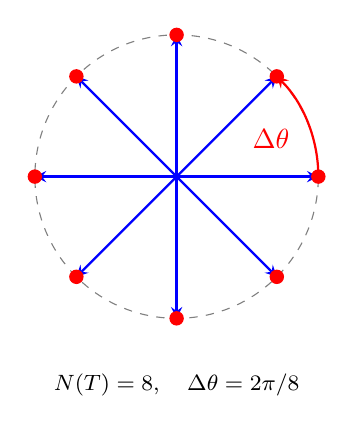
\begin{tikzpicture}[scale=1.2,>=stealth]
        \draw[gray, dashed] (0,0) circle (1.5);
        \foreach \k in {0,1,...,7} {
            \pgfmathsetmacro{\angle}{360*\k/8}
            \draw[->, thick, blue] (0,0) -- (\angle:1.5);
            \filldraw[red] (\angle:1.5) circle (2pt);
        }
        \draw[->, thick, red] (1.5,0) arc (0:45:1.5);
        \node[red] at (1.0,0.4) {$\Delta\theta$};
        \node[font=\footnotesize] at (0,-2.2) {$N(T)=8,\quad \Delta\theta=2\pi/8$};
    \end{tikzpicture}
    \caption{方向数与角分辨率。周期 $T$ 将圆周等分为 $T$ 个方向，相邻方向角间隔为 $\Delta\theta=2\pi/T$。}
    \label{fig:direction_resolution}
\end{figure}

\begin{definition}[通过方向数和角分辨率确定坐标点]\label{def:coordinate_by_width_bandwidth}
给定坐标点 $\mathbf{r} = (x, y) \neq \mathbf{0}$，辐角 $\theta = \arctan2(y, x)$。相位索引为
\[
k(\mathbf{r}; T) = \left\lfloor \theta \cdot T / (2\pi) \right\rfloor \bmod T.
\]
离散表示为
\[
\mathbf{r}_T = \|\mathbf{r}\| \cdot e^{i2\pi k/T}.
\]
\end{definition}

\begin{theorem}[离散向连续的极限过渡]\label{thm:discrete_to_continuous_limit}
设 $T_n \to \infty$。则
\[
\lim_{n \to \infty} \mathbf{r}_{T_n} = \mathbf{r}.
\]
\end{theorem}

\begin{proof}
离散化误差
\[
|\theta - 2\pi k/T_n| \le 2\pi/T_n \to 0.
\]
因此 $\mathbf{r}_{T_n}\to \mathbf{r}$。
\end{proof}

\begin{definition}[连续方向数与连续角分辨率]\label{def:continuous_width_bandwidth}
连续极限下，
\[
N_{\infty} = \infty, \qquad \Delta\theta_{\infty} = 0,
\]
满足极限对偶关系
\[
N_{\infty} \cdot \Delta\theta_{\infty} = 2\pi
\]
在广义意义下成立。
\end{definition}

\section{周期矢量场与三种微分算子的交换性}
\label{sec:periodic_vector_fields}

本章用梯度、散度、旋度与三个积分定理刻画了矢量场在平移、缩放、旋转三种基本变换下的行为。本节给出「周期」概念在矢量层面的入口：若矢量场在某个平移方向上周期，则三种微分算子保持该周期性；反之算子保持周期性并不蕴含原场周期。这条交换性是本章与全书「周期」主题的直接接合点。

\begin{definition}[周期标量场与周期矢量场]\label{def:periodic_vector_field}
设 $\mathbf a\in\mathbb R^3\setminus\{\mathbf 0\}$。称标量场 $f:\mathbb R^3\to\mathbb R$ 关于 $\mathbf a$ \textbf{周期}，若
\[
f(\mathbf x+\mathbf a)=f(\mathbf x),\qquad \forall \mathbf x\in\mathbb R^3 .
\]
称矢量场 $\mathbf F$ 关于 $\mathbf a$ 周期，若其三个分量均如此。使上式成立的全部 $\mathbf a$ 构成 $\mathbb R^3$ 的加法子群，记作 $\operatorname{Group}_{\mathrm{period}}(f)$（或 $\operatorname{Group}_{\mathrm{period}}(\mathbf F)$），称为该场的\textbf{具有周期轨道的群}。
\end{definition}

\begin{proposition}[三种微分算子与周期平移交换]\label{prop:operators_commute_period}
设 $f$ 为 $C^1$ 标量场、$\mathbf F$ 为 $C^1$ 矢量场，且均关于 $\mathbf a$ 周期。则
\begin{enumerate}[label=(\roman*)]
    \item 梯度：$(\nabla f)(\mathbf x+\mathbf a)=(\nabla f)(\mathbf x)$；
    \item 散度：$(\nabla\cdot\mathbf F)(\mathbf x+\mathbf a)=(\nabla\cdot\mathbf F)(\mathbf x)$；
    \item 旋度：$(\nabla\times\mathbf F)(\mathbf x+\mathbf a)=(\nabla\times\mathbf F)(\mathbf x)$。
\end{enumerate}
即三种微分算子都\textbf{保持周期平移下的不变性}。
\end{proposition}

\begin{proof}
(i) 设 $\mathbf e$ 为单位向量。由方向导数与链式法则，
\[
\mathbf e\cdot(\nabla f)(\mathbf x+\mathbf a)
=\frac{d}{dt}\Big|_{t=0}f(\mathbf x+\mathbf a+t\mathbf e)
=\frac{d}{dt}\Big|_{t=0}f(\mathbf x+t\mathbf e)
=\mathbf e\cdot(\nabla f)(\mathbf x),
\]
中间一步用到 $f(\mathbf y+\mathbf a)=f(\mathbf y)$（取 $\mathbf y=\mathbf x+t\mathbf e$）。由 $\mathbf e$ 任意即得 (i)。

(ii)(iii) 散度与旋度都是梯度分量的线性组合（见 \cref{def:divergence_vf} 与 \cref{def:curl_vf}），对 (i) 逐分量作相应的求和与差，即得结论。
\end{proof}

\begin{corollary}[沿周期方向的线积分为零]\label{cor:periodic_directional_integral_zero}
设 $f$ 为 $C^1$ 标量场、关于 $\mathbf a$ 周期。则
\[
\int_0^{1}\mathbf a\cdot\nabla f(\mathbf x+t\mathbf a)\,dt=0 .
\]
即：\textbf{周期标量场的梯度沿周期方向没有净增长}。
\end{corollary}

\begin{proof}
由链式法则，被积函数恰为 $\dfrac{d}{dt}f(\mathbf x+t\mathbf a)$，故积分等于 $f(\mathbf x+\mathbf a)-f(\mathbf x)=0$。
\end{proof}

\begin{remark}[与「周期」主题的接口]\label{rem:vf_period_interface}
命题 \ref{prop:operators_commute_period} 与推论 \ref{cor:periodic_directional_integral_zero} 给出本章在「周期」主题上的完整接口：
\[
\begin{aligned}
&\text{平移对称（周期）}\\
&\quad\Longrightarrow\ \text{微分算子保持该对称（守恒）}\\
&\quad\Longrightarrow\ \text{沿周期方向无净通量（闭合）}.
\end{aligned}
\]
该链条在「传播与演化」章用于周期介质中的 Bloch--Floquet 传播，在「电磁系统之周期结构」章用于周期边界条件下的 Maxwell 方程组。
须注意 (i) 的\textbf{逆命题不成立}：$\nabla f$ 关于 $\mathbf a$ 周期并不蕴含 $f$ 关于 $\mathbf a$ 周期——例如 $f(\mathbf x)=\mathbf e_1\cdot\mathbf x$ 的梯度为常向量场（关于一切 $\mathbf a$ 周期），而 $f$ 本身不周期。因此周期性判定必须在原场层面进行，不能只看其导数。
\end{remark}


\section*{本章七主题对照表}

\begin{center}
\renewcommand{\arraystretch}{1.3}
\begin{tabular}{>{\centering\arraybackslash}p{2.2cm}>{\centering\arraybackslash}p{11cm}}
\toprule
主题 & 本章对应 \\
\midrule
平移 & 梯度（对称中心 $0$） $\nabla$ 与方向导数；时间组相位梯度 \\
缩放 & 散度（对称中心 $1$） $\nabla\cdot$ 与平方反比律 \\
旋转 & 旋度（对称中心 $i$） $\nabla\times$ 与环量 \\
守恒 & 高斯定理与斯托克斯定理；空间组守恒律 \\
对称 & 微分算子与平移、缩放、旋转三类基本对称生成元的对应 \\
闭合 & 闭合曲线/曲面的环量与通量；投影算子的核 \\
周期 & 方向数与角分辨率的方向周期 \\
\bottomrule
\end{tabular}
\end{center}
\begin{table}[htbp]
    \centering
    \caption{本章结构的位置与前置依赖（便于核查与索引）}
    \label{tab:chapter_structure_map}
    \renewcommand{\arraystretch}{1.2}
    \footnotesize
    \setlength{\tabcolsep}{4pt}
    \begin{tabular}{@{}l >{\raggedright\arraybackslash}p{3.1cm} >{\raggedright\arraybackslash}p{10.3cm}@{}}
        \toprule
        \textbf{结构} & \textbf{主要落点} & \textbf{前置依赖（须先建立者）} \\
        \midrule
        定义 & 第 \ref{sec:trans_scale_rotate}、\ref{sec:nabla_properties} 节及后续各节 & 无（定义是一切的起点）\\
        引理 & 第 \ref{sec:trans_scale_rotate}、\ref{sec:nabla_properties} 节共 6 条 & 相应定义\\
        命题 & 第 \ref{sec:trans_scale_rotate}、\ref{sec:nabla_properties} 节及后续各节共 22 条 & 相应定义与引理\\
        定理 & 第 \ref{sec:trans_scale_rotate} 节起共 22 条 & 相应命题与引理\\
        证明 & 紧接每个定理与命题之后 & 被证对象\\
        推论 & 第 \ref{sec:nabla_properties}、\ref{sec:integral_theorems} 节起共 11 条 & 相应定理\\
        性质 & 投影模型与采样模型各节共 4 条 & 相应定义\\
        例子 & 反例分布于各节，共 26 条 & 相应定理与命题\\
        注释 & 用于界定适用范围与隐含假设，共 17 条 & 相应结论\\
        \bottomrule
    \end{tabular}
\end{table}

\section*{本章思考题}

\begin{enumerate}[leftmargin=3em, label=\textbf{题 \arabic*}]
    \item 证明引理 \ref{lem:translation_group}：平移群
    $(\mathcal{T}_n,\circ)$ 构成阿贝尔群，且
    \[
    (\mathcal{T}_n,\circ)\cong(\mathbb{R}^n,+).
    \]
    请写出复合封闭、结合律、单位元、逆元与同构的完整验证。

    \item 证明引理 \ref{lem:scaling_group}：缩放群
    $(\mathcal{S}_n,\circ)$ 构成阿贝尔群，且
    \[
    (\mathcal{S}_n,\circ)\cong(\mathbb{R}_{>0},\times).
    \]
    并说明为什么缩放因子必须取 $\lambda>0$——若允许 $\lambda=0$ 或 $\lambda<0$，
    分别会破坏什么性质。

    \item 证明命题 \ref{prop:similitude_group}：
    平移、缩放与旋转所生成的群等于保定向相似变换群
    \[
    \mathrm{Sim}^{+}(n)=\{\mathbf{x}\mapsto\lambda R\mathbf{x}+\mathbf{a}\mid
    \lambda>0,\;R\in SO(n),\;\mathbf{a}\in\mathbb{R}^n\}.
    \]
    请写出包含关系两个方向的证明，并说明为什么反射不属于该群。

    \item 验证例 \ref{ex:shear_anisotropic} 中剪切变换与各向异性缩放不属于相似群：
    \[
    A_t=\begin{pmatrix}1&t\\0&1\end{pmatrix},\qquad
    B=\operatorname{diag}(2,1).
    \]
    请分别计算 $A_t^{\mathsf T}A_t$ 与 $B^{\mathsf T}B$，
    证明二者均非标量矩阵，从而不属于 $\mathrm{Sim}^{+}(2)$。

    \item 证明命题 \ref{prop:divergence_flux_density}：
    散度是通量密度，
    \[
    \nabla\cdot\mathbf{F}(\mathbf{x}_0)
    =\lim_{r\to0^+}\frac{1}{|B_r|}\oint_{\partial B_r}\mathbf{F}\cdot\mathbf{n}\,dS.
    \]
    请利用球面上两个基本积分恒等式（引理 \ref{lem:sphere_flux_identities}）
    与一阶泰勒展开完成证明。

    \item 证明命题 \ref{prop:curl_circulation_density}：
    旋度是环量密度，
    \[
    (\nabla\times\mathbf{F}(\mathbf{x}_0))\cdot\mathbf{n}
    =\lim_{r\to0^+}\frac{1}{|D_r|}\oint_{\gamma_r}\mathbf{F}\cdot d\mathbf{r}.
    \]
    请取过 $\mathbf{x}_0$ 以 $\mathbf{n}$ 为法向的圆盘 $D_r$，
    将 $\mathbf{F}$ 作一阶展开并逐项积分完成证明。

    \item 证明定理 \ref{thm:infinitesimal_generators} 的三款结论：
    \begin{enumerate}[label=(\roman*)]
        \item 梯度与平移：$\frac{d}{dt}\big|_{t=0}f(\mathbf{x}+t\mathbf{a})=\mathbf{a}\cdot\nabla f(\mathbf{x})$；
        \item 散度与体积变化率：$\frac{d}{dt}\big|_{t=0}\operatorname{Vol}(\Phi_t(\Omega))=\int_\Omega\nabla\cdot\mathbf{F}\,dV$；
        \item 旋度与局部角速度：$\frac12(J-J^{\mathsf T})\mathbf{y}=\frac12(\nabla\times\mathbf{F})\times\mathbf{y}$。
    \end{enumerate}
    请分别用链式法则、Jacobi 公式与指标计算完成证明。

    \item 证明定理 \ref{thm:product_rules} 中的六条乘积法则：
    \begin{enumerate}[label=(\roman*)]
        \item $\nabla(fg)=f\nabla g+g\nabla f$；
        \item $\nabla\cdot(f\mathbf{F})=f(\nabla\cdot\mathbf{F})+\nabla f\cdot\mathbf{F}$；
        \item $\nabla\times(f\mathbf{F})=f(\nabla\times\mathbf{F})+\nabla f\times\mathbf{F}$；
        \item $\nabla\cdot(\mathbf{F}\times\mathbf{G})=\mathbf{G}\cdot(\nabla\times\mathbf{F})-\mathbf{F}\cdot(\nabla\times\mathbf{G})$；
        \item $\nabla\times(\mathbf{F}\times\mathbf{G})$ 的展开式；
        \item $\nabla(\mathbf{F}\cdot\mathbf{G})$ 的展开式。
    \end{enumerate}
    请用 Levi-Civita 符号 $\epsilon_{ijk}$ 与 $\epsilon$-收缩恒等式完成全部证明。

    \item 证明定理 \ref{thm:curl_grad_zero} 与定理 \ref{thm:div_curl_zero}：
    \[
    \nabla\times(\nabla f)=\mathbf{0},\qquad
    \nabla\cdot(\nabla\times\mathbf{F})=0.
    \]
    请说明两条恒等式的证明如何依赖于 Clairaut 混合偏导交换定理（引理 \ref{lem:clairaut}），
    并指出 $C^2$ 假设不可省略（参见反例 \ref{ex:clairaut_failure}）。

    \item 证明定理 \ref{thm:laplacian_decomp}：
    \[
    \nabla^2\mathbf{F}=\nabla(\nabla\cdot\mathbf{F})-\nabla\times(\nabla\times\mathbf{F}).
    \]
    请逐分量计算 $(\nabla^2\mathbf{F})_1$ 并验证与右端第一分量相等，
    说明两个混合偏导项因 Clairaut 定理相消。

    \item 证明格林公式（定理 \ref{thm:green_plane}）：
    设 $D$ 为有界闭区域，$\partial D$ 分段光滑，则
    \[
    \iint_D\left(\frac{\partial Q}{\partial x}-\frac{\partial P}{\partial y}\right)dx\,dy
    =\oint_{\partial D}(P\,dx+Q\,dy).
    \]
    请按“对 $y$-简单区域证明、对 $x$-简单区域证明、一般分段光滑边界求和”三步完成证明，
    并说明为什么相邻子区域的公共边积分两两相消。

    \item 证明旋度定理（定理 \ref{thm:stokes}）：
    \[
    \int_S(\nabla\times\mathbf{F})\cdot\mathbf{n}\,dS
    =\oint_{\partial S}\mathbf{F}\cdot d\mathbf{r}.
    \]
    请按“约化为 $z=h(x,y)$ 图曲面、化为 $D$ 上二重积分、对 $D$ 用格林公式、
    还原边界积分、一般分片光滑曲面求和”五步完成证明。

    \item 证明散度定理（定理 \ref{thm:divergence}）：
    \[
    \int_V(\nabla\cdot\mathbf{F})\,dV=\oint_{\partial V}\mathbf{F}\cdot\mathbf{n}\,dS.
    \]
    请按“长方体情形、$z$-简单区域、一般正则区域”三步完成证明，
    并说明为什么相邻子区域的公共面贡献两两相消。

    \item 验证反例 \ref{ex:slit_domain_counterexample}：
    在带缝平面 $\mathcal{M}=\mathbb{R}^2\setminus\{(x,0):x\ge0\}$ 上，
    矢量场
    \[
    \mathbf{F}(x,y)=\left(\frac{-y}{x^2+y^2},\frac{x}{x^2+y^2}\right)
    \]
    满足 $\nabla\times\mathbf{F}=\mathbf{0}$，但不存在标量势。
    请计算沿绕原点一周闭曲线的环量，并说明单连通性条件不可省略。

    \item 验证反例 \ref{ex:solenoidal_not_curl}：
    矢量场
    \[
    \mathbf{F}(\mathbf{x})=\frac{\mathbf{x}}{\|\mathbf{x}\|^3}
    \]
    在 $\mathbb{R}^3\setminus\{\mathbf{0}\}$ 上满足 $\nabla\cdot\mathbf{F}=0$，
    但不是任何矢量场的旋度。
    请计算穿过单位球面的通量，并说明为什么散度为零不是充分条件。

    \item 证明亥姆霍兹分解定理（定理 \ref{thm:helmholtz}）：
    适当衰减的矢量场可分解为无旋部分与无散部分之和：
    \[
    \mathbf{F}=-\nabla\phi+\nabla\times\mathbf{A}.
    \]
    请说明分解的存在性依赖于拉普拉斯算子的格林函数，
    并指出唯一性与显式积分公式需要衰减条件（参见反例 \ref{ex:helmholtz_decay_fails}）。

    \item 验证命题 \ref{prop:curvilinear_operators}：
    在正交曲线坐标系 $(\xi^1,\xi^2,\xi^3)$ 中，尺度因子为 $h_i$，
    \begin{enumerate}[label=(\roman*)]
        \item $\nabla f=\sum_i\frac{1}{h_i}\frac{\partial f}{\partial\xi^i}\mathbf{e}_i$；
        \item $\nabla\cdot\mathbf{F}=\frac{1}{h_1h_2h_3}\sum_i
              \frac{\partial}{\partial\xi^i}\left(\frac{h_1h_2h_3}{h_i}F_i\right)$；
        \item $(\nabla\times\mathbf{F})_1=\frac{1}{h_2h_3}
              \left[\frac{\partial(h_3F_3)}{\partial\xi^2}
              -\frac{\partial(h_2F_2)}{\partial\xi^3}\right]$。
    \end{enumerate}
    请分别写出球坐标与柱坐标下的具体表达式（例 \ref{ex:spherical_cylindrical}）。

    \item 证明平方反比定律（定理 \ref{thm:inverse_square}）：
    径向无源场若穿过任意包围中心的闭合曲面的总通量为常数 $\Phi_0$，
    则 $F(r)=\Phi_0/(4\pi r^2)$。
    请写出通量计算，并证明其逆命题（推论 \ref{cor:inverse_square_converse}）。

    \item 验证反例 \ref{ex:inverse_square_needs_const_flux}：
    取 $\mathbf{F}(\mathbf{r})=f(r)\hat{\mathbf{r}}$，
    其中 $f(r)=1/r^2$（$r\le1$），$f(r)=1/r^2+1$（$r>1$）。
    请计算 $r>1$ 时穿过球面的通量，验证它并非常数，
    并说明“通量为常数”是一条独立前提，而非无源加球对称的自动推论。

    \item 综合题：结合三种基本变换（定义 \ref{def:translation_map}、\ref{def:scaling_map}、
    \ref{def:rotation_map}）、三种微分算子（定义 \ref{def:gradient_vf}、
    \ref{def:divergence_vf}、\ref{def:curl_vf}）
    与三个积分定理（定理 \ref{thm:green_plane}、\ref{thm:stokes}、\ref{thm:divergence}），
    说明矢量分析如何把周期数学的三大对称中心——加法对称中心 $0$、
    乘法对称中心 $1$、旋转对称中心 $i$——在向量场层面具体化。
    请分别指出哪些积分定理对应守恒律，并说明三组对象之间的层次差异
    （参见注 \ref{rem:centres_and_two_triples}）。
\end{enumerate}

